%%%%%%%%%%%%%%%%%%%%%%%%%%%%%%%%%%%%%%%%%
% Masters/Doctoral Thesis 
% LaTeX Template
% Version 2.5 (27/8/17)
%
% This template was downloaded from:
% http://www.LaTeXTemplates.com
%
% Version 2.x major modifications by:
% Vel (vel@latextemplates.com)
%
% This template is based on a template by:
% Steve Gunn (http://users.ecs.soton.ac.uk/srg/softwaretools/document/templates/)
% Sunil Patel (http://www.sunilpatel.co.uk/thesis-template/)
%
% Template license:
% CC BY-NC-SA 3.0 (http://creativecommons.org/licenses/by-nc-sa/3.0/)
%
%%%%%%%%%%%%%%%%%%%%%%%%%%%%%%%%%%%%%%%%%

%----------------------------------------------------------------------------------------
%	PACKAGES AND OTHER DOCUMENT CONFIGURATIONS
%----------------------------------------------------------------------------------------

\documentclass[
12pt, % The default document font size, options: 10pt, 11pt, 12pt
oneside, % Two side (alternating margins) for binding by default, uncomment to switch to one side
english, % ngerman for German
onehalfspacing, % Single line spacing, alternatives: onehalfspacing or doublespacing, singlespacing
%draft, % Uncomment to enable draft mode (no pictures, no links, overfull hboxes indicated)
%nolistspacing, % If the document is onehalfspacing or doublespacing, uncomment this to set spacing in lists to single
%liststotoc, % Uncomment to add the list of figures/tables/etc to the table of contents
%toctotoc, % Uncomment to add the main table of contents to the table of contents
%parskip, % Uncomment to add space between paragraphs
%nohyperref, % Uncomment to not load the hyperref package
headsepline, % Uncomment to get a line under the header
%chapterinoneline, % Uncomment to place the chapter title next to the number on one line
%consistentlayout, % Uncomment to change the layout of the declaration, abstract and acknowledgements pages to match the default layout
]{MastersDoctoralThesis} % The class file specifying the document structure

\usepackage[utf8]{inputenc} % Required for inputting international characters
\usepackage[T1]{fontenc} % Output font encoding for international characters

\usepackage{mathpazo} % Use the Palatino font by default

\usepackage[backend=bibtex,style=authoryear,natbib=true]{biblatex} % Use the bibtex backend with the authoryear citation style (which resembles APA)

\addbibresource{library.bib} % The filename of the bibliography

\usepackage[autostyle=true]{csquotes} % Required to generate language-dependent quotes in the bibliography
\usepackage{{booktabs}}
\usepackage{multirow}
%----------------------------------------------------------------------------------------
%	MARGIN SETTINGS
%----------------------------------------------------------------------------------------

\geometry{
	paper=a4paper, % Change to letterpaper for US letter
	inner=2.5cm, % Inner margin
	outer=3.8cm, % Outer margin
	bindingoffset=.5cm, % Binding offset
	top=1.5cm, % Top margin
	bottom=1.5cm, % Bottom margin
	%showframe, % Uncomment to show how the type block is set on the page
}

%----------------------------------------------------------------------------------------
%	THESIS INFORMATION
%----------------------------------------------------------------------------------------

\thesistitle{The effect of government support during the COVID-19 pandemic: Firm-level evidence from Germany} % Your thesis title, this is used in the title and abstract, print it elsewhere with \ttitle
\supervisor{Dr. Simon \textsc{Munzert}} % Your supervisor's name, this is used in the title page, print it elsewhere with \supname
\examiner{} % Your examiner's name, this is not currently used anywhere in the template, print it elsewhere with \examname
\degree{Master of Data Science for Public} % Your degree name, this is used in the title page and abstract, print it elsewhere with \degreename
\author{Marco \textsc{Schildt}} % Your name, this is used in the title page and abstract, print it elsewhere with \authorname
\addresses{} % Your address, this is not currently used anywhere in the template, print it elsewhere with \addressname

\subject{} % Your subject area, this is not currently used anywhere in the template, print it elsewhere with \subjectname
\keywords{} % Keywords for your thesis, this is not currently used anywhere in the template, print it elsewhere with \keywordnames
\university{\href{https://www.hertie-school.org}{Hertie School}} % Your university's name and URL, this is used in the title page and abstract, print it elsewhere with \univname
\department{} % Your department's name and URL, this is used in the title page and abstract, print it elsewhere with \deptname
\group{} % Your research group's name and URL, this is used in the title page, print it elsewhere with \groupname
\faculty{} % Your faculty's name and URL, this is used in the title page and abstract, print it elsewhere with \facname

\AtBeginDocument{
\hypersetup{pdftitle=\ttitle} % Set the PDF's title to your title
\hypersetup{pdfauthor=\authorname} % Set the PDF's author to your name
\hypersetup{pdfkeywords=\keywordnames} % Set the PDF's keywords to your keywords
%\hypersetup{citecolor=black}
%\hypersetup{urlcolor=black}
}

\begin{document}

\frontmatter % Use roman page numbering style (i, ii, iii, iv...) for the pre-content pages

\pagestyle{plain} % Default to the plain heading style until the thesis style is called for the body content

%----------------------------------------------------------------------------------------
%	TITLE PAGE
%----------------------------------------------------------------------------------------

\begin{titlepage}
\begin{center}

\vspace*{.06\textheight}
{\scshape\LARGE \univname\par}\vspace{1.5cm} % University name
\textsc{\Large Master Thesis}\\[0.5cm] % Thesis type

\HRule \\[0.4cm] % Horizontal line
{\huge \bfseries \ttitle\par}\vspace{0.4cm} % Thesis title
\HRule \\[1.5cm] % Horizontal line
 
\begin{minipage}[t]{0.4\textwidth}
\begin{flushleft} \large
\emph{Author:}\\
{\authorname} % Author name - remove the \href bracket to remove the link
\end{flushleft}
\end{minipage}
\begin{minipage}[t]{0.4\textwidth}
\begin{flushright} \large
\emph{Supervisor:} \\
{\supname} % Supervisor name - remove the \href bracket to remove the link  
\end{flushright}
\end{minipage}\\[3cm]
 
\vfill

\large \textit{A thesis submitted in fulfillment of the requirements\\ for the degree of \degreename}\\[0.3cm] % University requirement text
%\textit{in the}\\[0.4cm]
%\groupname\\\deptname\\[2cm] % Research group name and department name
 
\vfill

{\large \today}\\Wordcount: X.XXX\\[4cm] % Date
%\includegraphics{Logo} % University/department logo - uncomment to place it
 
\vfill
\end{center}
\end{titlepage}


\cleardoublepage


%----------------------------------------------------------------------------------------
%	ABSTRACT PAGE
%----------------------------------------------------------------------------------------
\def\abstractname{Executive Summary}
\begin{abstract}

\addchaptertocentry{\abstractname} % Add the abstract to the table of contents
\noindent
The Thesis Abstract is written here (and usually kept to just this page). 
The page is kept centered vertically so can expand into the blank space above the title too\ldots

\end{abstract}


%----------------------------------------------------------------------------------------
%	LIST OF CONTENTS/FIGURES/TABLES PAGES
%----------------------------------------------------------------------------------------
\hypersetup{linkcolor=black}
\tableofcontents % Prints the main table of contents

\listoffigures % Prints the list of figures

\listoftables % Prints the list of tables

%----------------------------------------------------------------------------------------
%	ABBREVIATIONS
%----------------------------------------------------------------------------------------

\begin{abbreviations}{ll} % Include a list of abbreviations (a table of two columns)

\textbf{ATT} & \textbf{A}verage \textbf{T}treatment Effect on the \textbf{T}reated\\
\textbf{EU COM} & \textbf{EU}ropean \textbf{COM}mission\\
\textbf{SMEs} & \textbf{S}mall and \textbf{M}edium-sized \textbf{E}nterprises\\




\end{abbreviations}




%----------------------------------------------------------------------------------------
%	THESIS CONTENT - CHAPTERS
%----------------------------------------------------------------------------------------

\mainmatter % Begin numeric (1,2,3...) page numbering

\pagestyle{thesis} % Return the page headers back to the "thesis" style

% Include the chapters of the thesis as separate files from the Chapters folder
% Uncomment the lines as you write the chapters



% Chapter Template

\chapter{Introduction to the government support in Germany} % Main chapter title

\label{Chapter1} % Change X to a consecutive number; for referencing this chapter elsewhere, use \ref{ChapterX}


%----------------------------------------------------------------------------------------
%	No SubsECTION 
%----------------------------------------------------------------------------------------


The Covid-19 pandemic has severely affected the entire world with many devastating consequences. Businesses in many parts of the economy were struggling to survive due to shocks in demand, lockdowns from governments and disrupted supply chains \parencite{eu_com_temporary_2020}.

To sustain the economy and prevent businesses them from bankruptcy during the pandemic, the German government responded with a range of policies. Beside the various measures like labor cost subsidies, temporary changes in the insolvency law and tax reliefs, the financial support through grants and loans was unprecedented. The financial support was available for businesses in all sizes that affected by the pandemic ranging from self-employed individuals to small and medium-sized enterprises (SMEs) up to very large companies. From spring 2020 to summer 2022, grants, loans, recapitalizations and guarantees alone accounted for a total of around EUR 130 billion \parencite{bmwk_uberblickspapier_2022}. 


A fiscal effort of this magnitude is inconceivable under normal conditions. Usually, governments are not permitted to provide extensive subsidies, due to concerns of distorting competing in the European single market \parencite{claici_european_2022}. The permissibility of subsidies is comprehensively regulated by European state aid laws. Before a subsidy is considered permissible under this legal framework an assessment of its necessity, incentive effect, proportionality and effect on trade and competition is needed \parencite{claici_european_2022}. In light of the ongoing pandemic, the EU relaxed rules on subsidies by introducing the Temporary Framework for State aid measures to support the economy in the current COVID-19 outbreak, by which provided national governments more freedom in order to come up with quick and extensive policy responses to support businesses \parencite{eu_com_temporary_2020}.

As part of the framework the German government had to justify the financial support measures by laying out the necessity, the appropriateness and proportionality to remedy the impact of the pandemic in the economy. Defining and deciding on the appropriateness as well as proportionality of support measures is a complex and challenging task. Due to the unpredictable scale of the pandemic, uncertainty is immense. On the other hand, the effect of support measures is nothing trivial to estimate, given that their scale was unprecedented. To ensure that the support measures are effective, efficient, a good understanding is inevitable.

The financial support measures introduced by the German government can mainly be categorized into the groups grants and loans. Grants are funds provided by the government to businesses that are not needed to be repaid. Grants are usually subject to the terms and conditions, but do not require any consideration in return. Whereas financial support measures based on loans have to be repaid, like standard bank loans. The advantage over a normal credit transaction are beneficial conditions that a company would not have received under normal circumstances from a bank. Especially not in a time where the company’s future is uncertain and linked to the further development of the pandemic. 

From the companies' point of view, both types of aid have the immediate effect of a liquidity injection, meaning that additional cash is available. However, in the long-term perspective the repayment obligation of loans is contrasting the effect of grants by the fact that a firm will have to service the debt and interest of the loan, regardless of whether the pandemic is over or not.

This thesis is organized as follows. After an introduction to the government support in Germany in section 1, section 2 provides an overview of the general effects of COVID-19 pandemic on business as well as the existing impact assessments of government support.
Section 3 presents the data and section 4 explains the utilized methodologies. In Section 5, the causal evidence of the aid measures is shown. Section 6 covers the policy implications and concludes.



\begin{table}
\caption{Overview of support instruments}
\label{tab:treatments}
\centering
\begin{tabular}{lr}
\toprule
                   Beihilfeinstrument &               aid \\
\midrule
Andere Formen der Kapitalintervention &  9,017,729,574.33 \\
                           Bürgschaft &  1,144,042,410.02 \\
              Eigenkapitalinstrumente &  2,419,881,701.00 \\
      Kredite/rückzahlbare Vorschüsse &    753,217,635.27 \\
            Sonstiges (bitte angeben) & 14,244,894,962.69 \\
               Zinsgünstiges Darlehen & 10,500,942,385.00 \\
                         Zinszuschuss &  9,383,307,910.00 \\
                             Zuschuss & 24,959,647,770.34 \\
\bottomrule
\end{tabular}
}

\end{table}
    

%\caption{The effects of treatments X and Y on the four groups studied.}


% Chapter Template

\chapter{Literature Review} % Main chapter title

\label{Chapter2} % Change X to a consecutive number; for referencing this chapter elsewhere, use \ref{ChapterX}

%----------------------------------------------------------------------------------------
%	SECTION 1
%----------------------------------------------------------------------------------------

\section{Pandemic effects}

The negative consequences of the COVID-19 pandemic on the economy have become evident in many areas. Many businesses were severely affected by drops in demand and through lockdowns ordered by authorities. When business operations are halting while costs like rent or personal costs continue occurring the pandemic shock eventually leads to negative cash flows for many firms \parencite{fernandez-cerezo_firm-level_2021}.
Depending on the affectedness of the business, the liquidity reserves will inevitably deteriorate and eventually liquidity shortfalls are inescapable with negative cash flows \parencite{puhr_have_2021}.
Although the demand of liquidity is individual for every company, a simulation study from Italy quantified the total liquidity deficit of all Italian SMEs caused by the Covid-19 shock to 83.7 billion Euros at the end of 2020 \parencite{bellucci_consequences_2022}. 
In comparison for the Belgian corporate sector, in a scenario without policy interventions, the drop in liquidity by September 2020 is quantified with 28.2 billion Euros \parencite{tielens_belgian_2020}. 

Empirical results from Tielens et al. (2020) suggest that in Belgium even businesses that used to be profitable require a large amount of additional financing to offset their liquidity shortfall.

Without a return of profits, firms are in need of liquidity injection to, either through additional equity or via debt. For smaller unlisted firms it is usually not possible to easily raising equity, therefore they usually left with the debt option and rely on credits from banks \parencite{pagano_covid-19_2022}. Pagano and Zechner \parencite*{pagano_covid-19_2022} analyzed the effects of covid 19 on companies’ financial performance in the EU. Their evidence suggests differences in the effects between large firms and small and medium sized enterprises. By comparing the years 2019 and 2020 the authors found that smaller companies tend to increase their ratio of total debt to total assets (debt-ratio) whereas, large companies also increase their leverage, but significantly less. Regarding liquidity, their findings suggest that small and medium sized enterprises increased their cash-to-total-assets-ratio more than large companies. Small companies did so even more than medium sized ones. However, the authors could only speculate over the reason behind of this observation. Plausible reasons were precautionary cash hording and greater risk aversion. Additionally, the authors raise the theory that smaller companies were able to raise cash more easily due to the claim, that loan guarantee programs favored small firms. However, the analyzed sample of small and medium sized enterprises was not representative of any specific industry, nor of aid recipients.

However, credits from banks, if obtainable, increases the firms leverage and could make the firm vulnerable to new liquidity shortfalls. And additional leverage only prevents from insolvency if there is a prospect that future cash flows will enable a firm to service the additional debt. Regarding the capital structure, increased leverage means a weaker equity ratio. An early Survey study from September 2020 analyzed the implications of the pandemic crisis on the equity of Germany companies and reported that for most companies the equity ratio did not change, however a strong sectoral heterogeneity with travel and gastronomy having a reduction in the equity ratio between 1.8 \% and 1.5 \% \parencite{peichl_eigenkapitalentwicklung_2021}. In Spain a survey looked at the indebtedness as well as the cash ratio of enterprises and reported findings that support the heterogeneity of the covid 19 shock across firms and, that the impact was larger for small, young and less productive firms located in urban areas \parencite{fernandez-cerezo_firm-level_2021}. Further support for the heterogeneity of the impact of the COVID-19 crisis on firms’ sales and costs came from Belgium \parencite{dhyne_belgian_2021}.

A simulation on 14 relatively well-covered European countries estimated that an increase in the financial debt of companies has on average a negative impact on the growth of investment after the crisis, indicating negative long-term effects increased leverage \parencite{demmou_insolvency_2021}.



%----------------------------------------------------------------------------------------
%	SECTION 2
%----------------------------------------------------------------------------------------

\section{Government support effects}

Policy intervention to "prevent” the effects and save businesses for a fast economic recovery.
First assessments were modeling approaches.
Already lots of early assessments of state aid, also at a firm level.
For getting a better understanding on the effect of aid schemes in Germany a paper analyses the effect of a company’s cost structure on the effectives of aid measures (Bischof, Karlsson, Rostam-Aschar, Simon, 2021). 
This paper assumes that companies within the same sector have a similar cost structure. 
Since aid in Germany is based on the cost structure of companies, the authors conclude that based on the generalized approach of aid schemes, the effectiveness of aid is varying between business sectors.
% Chapter Template

\chapter{Data Sources} % Main chapter title

\label{ChapterX} % Change X to a consecutive number; for referencing this chapter elsewhere, use \ref{ChapterX}

%----------------------------------------------------------------------------------------
%	SECTION 1
%----------------------------------------------------------------------------------------

\section{Data on Government support}

Research unambiguous concluded that COVID-19 crisis negatively influenced the economy in countries around the world. Many businesses were severely affected by drops in demand and lockdowns by the authorities. The pandemic shock leads to negative cash flows for many firms (Fernández-Cerezo et al. 2021). Depending on the affectedness of the business and the cash holding, liquidity shortfalls are inescapable. 
Without continuation of their business and positive cash flows, firm’s equity and the liquidity (cash and bank) positions will inevitably deteriorate. At some point, firms are in need of Liquidity injection, either through additional equity or via debt. However, debt, if obtainable, increases the firms leverage and could make the firm vulnerable to new liquidity shortfalls. And, additional leverage only prevents from insolvency if there is a prospect that future cash flows will enable a firm to service the additional debt.
The effect of the COVID-19 outbreak is widely described as an economic shock,

Pagano and Zechner empirically analyzed the effects of covid 19 on companies’ financial performance in the EU (2022). Their finding shows significant differences in the effects between large firms and small and medium sized enterprises. 
By comparing the year 2019 and 2020 the authors found that smaller companies tend to increase their ratio of total debt to total assets (debt-ratio) whereas, large companies also increase their leverage, but significantly less.
Regarding liquidity, small and medium sized enterprises increased their cash to total assets ratio more than large companies. Small companies did so even more than medium sized ones. However, the authors could only speculate over the reason behind of this observation. Plausible reasons were precautionary cash hording and greater risk aversion. Additionally, the authors raise the theory that smaller companies were able to raise cash more easily due to the claim, that loan guarantee programs favored small firms. However, the analyzed sample of small and medium sized enterprises was not representative of any specific industry, nor of aid recipients. 
A study by Peichl et al. analyses the implications of the pandemic crisis on the equity of Germany companies (2021). They found in their early survey from September that for most companies the equity ratio did not change, however a strong sectoral heterogeneity with travel and gastronomy having a reduction in the equity ratio between 1.8 % and 1.5 %.
(Tielens et al. 2021) conducted a significant short-run impact on firms’ liquidity buffers in Belgium by the covid 19 Pandemic. (Narrow liquidity ratio) And heterogeneous impact of the COVID-19 crisis on the cash position of Belgian firms in comparison to a business-as-usual counterfactual.
In Spain a survey looked at amongst other indicators looked at indebtedness and cash ratio of enterprises. Findings support the heterogeneity of the covid 19 shock across firms and that the impact was larger for small, young and less productive firms located in urban areas. (Fernández-Cerezo et al. 2021).
Heterogeneous impact of the COVID-19 crisis on firms’ sales and costs, see Dhyne and Duprez (2021)




%----------------------------------------------------------------------------------------
%	SECTION 2
%----------------------------------------------------------------------------------------

\section{Company level financial information}

Policy intervention to "prevent” the effects and save businesses for a fast economic recovery.
First assessments were modeling approaches.
Already lots of early assessments of state aid, also at a firm level.
For getting a better understanding on the effect of aid schemes in Germany a paper analyses the effect of a company’s cost structure on the effectives of aid measures (Bischof, Karlsson, Rostam-Aschar, Simon, 2021). 
This paper assumes that companies within the same sector have a similar cost structure. 
Since aid in Germany is based on the cost structure of companies, the authors conclude that based on the generalized approach of aid schemes, the effectiveness of aid is varying between business sectors.
% Chapter Template

\chapter{Methods} % Main chapter title

\label{Chapter4} % Change X to a consecutive number; for referencing this chapter elsewhere, use \ref{ChapterX}

%----------------------------------------------------------------------------------------
%	SECTION 1
%----------------------------------------------------------------------------------------

\section{Balance Sheet Ratios}

Even though balance sheets offer a reporting date view on the firm’s financial information and can’t reflect events or extreme situations during a fiscal year, they provide comparable view on companies that is standardized by accounting standards. To achieve comparability of the financial situation of companies despite their different sizes, the collected balance sheet data is used to calculate ratios. With that available financial a selection of balance sheet ratios is calculated to provide a consistent indication of a firm’s situation in terms of liquidity and leverage. The ratios are calculated for each beneficiary of government support for each available year between 2018 and 2022. Calculations are shown in table \ref{tab:RatioCalc}.


\subsection{Liquidity Ratios}

Liquidity ratios are chosen to measure a firm’s financial position to meet its obligations in the short run. As outlined in chapter \ref{Chapter1}the pandemic shock had a significant effect on companies’ liquidity and was a key consideration for the EU to loosen state aid regulation and enable large scale support measures \parencite{eu_com_temporary_2020}.

The first and most representative liquidity ratio is the cash ratio, comparing the most liquid asset, cash holdings, to the total assets of a firm. Cash is the starting buffer against running costs in a crisis shock. Although usually the current liabilities are used instead of the total assets, with the available data total assets serve as a more robust denominator that has been utilizes in similar research \parencite{fernandez-cerezo_firm-level_2021, costa_state-aids_2021,igan_shot_2023}.

\subsection{Solvency Ratios}

The other factor of interest is the indebtedness of firm in context with the pandemic and the remedy measures. The indebtedness, or also leverage, of a firm has implications that are rather relevant in the long-term, since debt payments are long term obligations that need to be serviced by cash flows. High levels of debt can challenge a company and can reduce profits. 
The debt-to-asset and the equity ratio compare the respective capital to the total assets and are behaving in opposite directions. The debt-to-equity ratio give a magnified picture on the companies leverage compared to the debt-to-asset ratio. For the simplification purposes negative ratios were omitted since result either from errors in the data parsing process or from exceptional cases like loss transfer agreements with parent companies. 

\begin{table}[]
    \caption{The calculation of Balance Sheet Ratios.}
    \label{tab:RatioCalc}
    \centering
    \def\arraystretch{1.5}
    \begin{tabular}{@{}lll@{}}
    \toprule
    Category                   & Ratio                & Calculation \\ \midrule
    \multirow{3}{*}{Liquidity} & Cash Ratio           & $\frac{Cash}{Total Assets}$ \\ %\cmidrule(l){2-3} 
                                & Quick Ratio          & $\frac{Current Assets-Inventory}{Current Liabilities}$ \\ %\cmidrule(l){2-3} 
                                & Current Ratio        & $\frac{Current Assets}{Current Liabilities}$ \\ \midrule
    \multirow{3}{*}{Liability} & Debt-to-Equity Ratio & $\frac{Debt}{Equity}$ \\ %\cmidrule(l){2-3} 
                                & Equity Ratio         & $\frac{Equity}{Total Assets}$ \\ %\cmidrule(l){2-3} 
                                & Debt-to-Assets Ratio & $\frac{Debt}{Total Assets}$ \\ \bottomrule
    \end{tabular}
    \end{table}

%----------------------------------------------------------------------------------------
%	SECTION 2
%----------------------------------------------------------------------------------------

\section{Diff and Diff}

Policy intervention to "prevent” the effects and save businesses for a fast economic recovery.
First assessments were modeling approaches.
Already lots of early assessments of state aid, also at a firm level.
For getting a better understanding on the effect of aid schemes in Germany a paper analyses the effect of a company’s cost structure on the effectives of aid measures (Bischof, Karlsson, Rostam-Aschar, Simon, 2021). 
This paper assumes that companies within the same sector have a similar cost structure. 
Since aid in Germany is based on the cost structure of companies, the authors conclude that based on the generalized approach of aid schemes, the effectiveness of aid is varying between business sectors.


%----------------------------------------------------------------------------------------
%	SECTION 3
%----------------------------------------------------------------------------------------

\section{Causal Curve}

Policy intervention to "prevent” the effects and save businesses for a fast economic recovery.
First assessments were modeling approaches.
Already lots of early assessments of state aid, also at a firm level.
For getting a better understanding on the effect of aid schemes in Germany a paper analyses the effect of a company’s cost structure on the effectives of aid measures (Bischof, Karlsson, Rostam-Aschar, Simon, 2021). 
This paper assumes that companies within the same sector have a similar cost structure. 
Since aid in Germany is based on the cost structure of companies, the authors conclude that based on the generalized approach of aid schemes, the effectiveness of aid is varying between business sectors.
% Chapter Template

\chapter{Results} % Main chapter title

\label{Chapter5} % Change X to a consecutive number; for referencing this chapter elsewhere, use \ref{ChapterX}

%----------------------------------------------------------------------------------------
%	SECTION 1
%----------------------------------------------------------------------------------------

\section{Data insights on beneficiaries}
\label{BSratio}

\subsection{Liquidity}

In Figure \ref{fig:Ratios} the calculated ratios for all companies of the dataset are shown with boxplots for the years 2018-202. With the median, shown as the middle line in the box, the first and the third quartile, boxplots allow a simple comparison between the years that is not sensitive for outliers. The three observed liquidity ratios show an increase in liquidity in 2020 and 2021 compared to the pre-pandemic years, indicating that companies were holding relatively more cash at the year-end since the pandemic. 
Overall, the observations are in line with a study conducted by the German Federal Bank that also reported an increase in the average cash ratio for the whole population of German companies in 2020 as well as in 2021 \parencite{deutsche_bundesbank_jahresabschlussstatistik_2022}. For example, for SME corporations the study reported a change in the cash ratio from 0.104 (2019) to 0.110 (2020). For the current ratio and quick ratio, the same trend was reported. Further support for an increase in the quick ratio comes from another study by \parencite{bley_mittelstand_2022}. Although the exact ratios are varying between studies, there is strong support for the general trend of increasing liquidity in 2020 and 2021.
What also can be seen in Figure \ref{fig:Ratios} is that the whiskers of the boxplots are longer in the pandemic years, showing the heterogeneity of liquidity levels for firms. Considering that the ratios only reflect the status of the cutoff date, this can also be an indicator that the liquidity levels of firms are more volatile than before the pandemic which could be caused by forecasting difficulties in the liquidity planning during the pandemic. 


\subsection{Solvency}

Solvency ratios are showing a less clear trend after the COVID-19 pandemic. Although minimal, the opposite trends in the equity ratio and debt-to-asset ratio are as expected. The only visible change happened in 2020, while in 2021 the ratios are very similar to 2018 and 2019. The change in the debt-to-asset ratio is amplified in the debt-to-equity ratio, as expected. Survey Data from the KFW found an Equity Ratio of 0.318 in 2019, a decrease to 0.301 in 2020, and a recovery to 0.314 in 2021 \parencite{kfw_kfw-mittelstandspanel_2022}. For very small companies with less than 10 employees, the drop in 2020 was stronger, and the recovery in 2021 was above pre-pandemic levels. On the other hand, the survey reported
that larger companies did not have a recovery after the first crisis year and decreased their Equity Ratio in 2021 on average further. 
This could indicate that the recovery of the indebtedness of beneficiaries in 2021 might have been driven by smaller companies. Similar observations were reported by the German Federal Bank were the debt-to-asset ratio for SME corporations decreased in 2020 \parencite{deutsche_bundesbank_jahresabschlussstatistik_2022}.



\begin{figure}
\centering
\makebox[\textwidth][c]{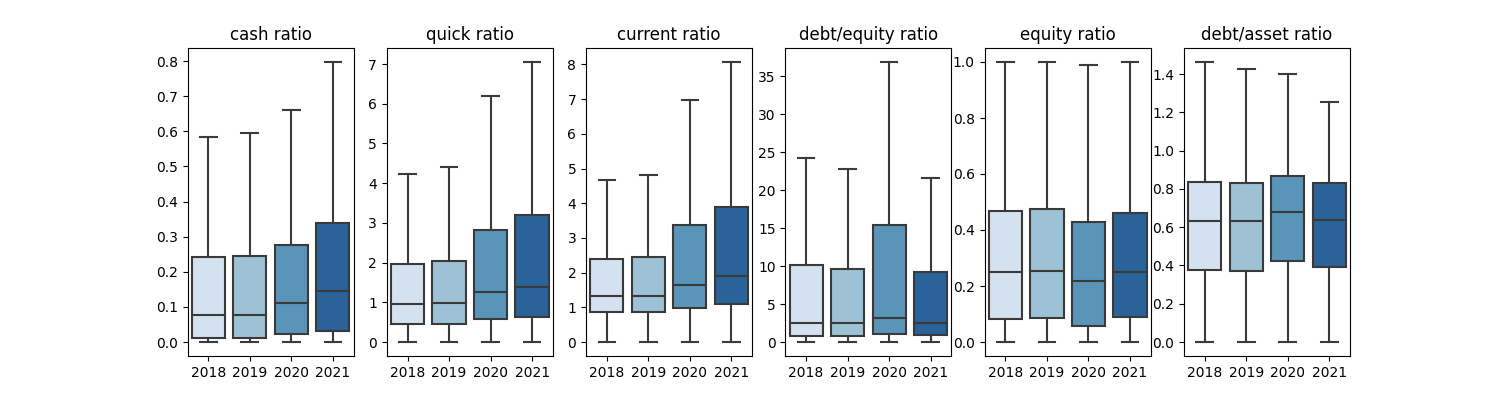
\includegraphics[width=1.3\columnwidth]{Figures/chart_ratios}}%

\decoRule
\caption[Indicators of liquidity and solvency 2019-2021]{Boxplots with balance sheet ratios from the obtained dataset. Extreme outliers above the maximum values are not shown.}
\label{fig:Ratios}
\end{figure}






\subsection{Insolvencies of beneficiaries}


In total 953 insolvent firms were identified representing a share of 0.92 \% of all beneficiaries of pandemic aid from the transparency database, as shown in Table \ref{tab:InsBySize}. A further breakdown reveals that the share of SMEs is significantly lower than their larger counterparts. Since the transparency database only provides very few beneficiaries with aid payments below 100.000 EUR, smaller companies with aid below the threshold are not well represented. Therefore, the numbers only give an indication.

\begin{table}
\caption{Share of insolvent aid  beneficiaries by size}
\label{tab:InsBySize}
\centering

\def\arraystretch{1.2}
\centering
\begin{tabular}{lrrl}
\toprule
           size &  aid beneficiaries &  insolvent & share \\
\midrule
           SMEs &              78077 &        526 & 0.67\% \\
Large companies &              25259 &        427 & 1.69\% \\
          Total &             103336 &        953 & 0.92\% \\
\bottomrule
\end{tabular}
}

\end{table}

In the next step the industries of insolvent beneficiaries were analyzed. The results for the most represented industries are presented in Table \ref{tab:InsByIndustry_short}. A more comprehensive table with more industries is in Appendix \ref{AppendixB}. The findings show that food and beverage service activities are the industry with the most beneficiaries, but only have a share of 0.58 \% of insolvencies that well below the average. 

Similarly, the accommodation sector is highly represented. With only 24 insolvencies out of 9.885 recipients, it has the lowest share amongst the most represented industries. On the higher end are specialized construction activities with a share of 1.66 \%. The closely related construction building sector has an even higher share with 2.97 \%, but is less represented and therefore only shown in the appendix. Partially, even higher shares are present in the data, but only in underrepresented industries. 

\begin{table}
    \caption{Share of insolvent aid  beneficiaries by industry}
    \label{tab:InsByIndustry_short}
    \centering
    \def\arraystretch{1}
    \centering
    \begin{tabular}{lrrl}
\toprule
                                industry &  beneficiaries &  insolvent & share \\
\midrule
    Food and beverage service activities &          15173 &         88 & 0.58\% \\
Retail trade, except of motor vehicles a &           8810 &         84 & 0.95\% \\
     Specialised construction activities &           4103 &         68 & 1.66\% \\
Wholesale trade, except of motor vehicle &           5396 &         56 & 1.04\% \\
Manufacture of fabricated metal products &           3105 &         40 & 1.29\% \\
Office administrative, office support an &           3040 &         28 & 0.92\% \\
Sports activities and amusement and recr &           5232 &         27 & 0.52\% \\
                           Accommodation &           9885 &         24 & 0.24\% \\
Wholesale and retail trade and repair of &           3525 &         17 & 0.48\% \\
\bottomrule
\end{tabular}
}

    \small  Notes: The table shows industries with more than 3000 beneficiaries and is sorted by insolvencies. The industry names are truncated after 40 characters.

\end{table}




\subsection{Ratios of insolvencies}

Next, the ratios of insolvent beneficiaries are analyzed and compared to the other beneficiaries. For the comparison, the cash ratio and the debt-to-asset ratio are chosen to analyze the liquidity and solvency. Figure \ref{fig:RatiosInsolvency} shows the already for section \ref{BSratio} used boxplot, but grouped into a solvent (light blue) and insolvent by the spring of 2023 (darker blue). For the liquidity ratio, a clear discrepancy can be observed throughout all periods. The group of companies that later got insolvent has already before 2020 significantly less liquidity than the other group. However, in 2020 and 2021 their cash ratio is also increasing, like the solvent group.
The debt-to-asset ratio comparison also shows a clear gap between both groups. The companies which are later becoming insolvent have higher leverage before and after the start of the pandemic. 

\begin{figure}
    \centering
    \makebox[\textwidth][c]{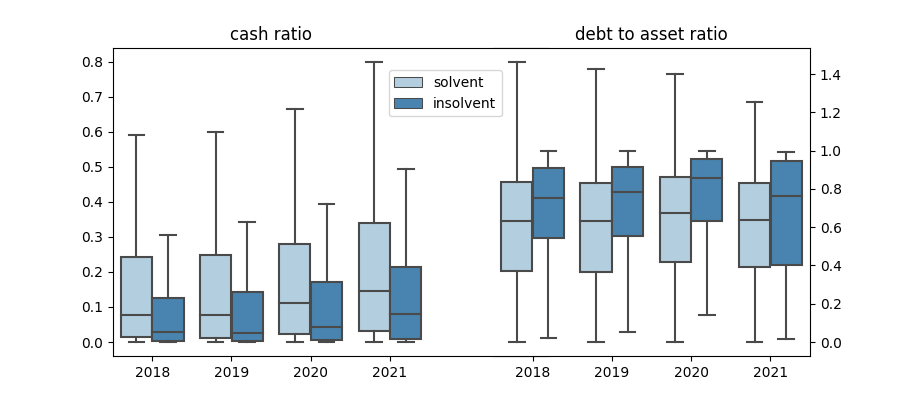
\includegraphics[width=1.2\columnwidth]{Figures/chart_ratios_insolvence}}%
    
    \decoRule
    \caption[Liquidity and solvency of insolvent beneficiaries]{Boxplot with balance sheet ratios from the obtained dataset.}
    \label{fig:RatiosInsolvency}
\end{figure}





%----------------------------------------------------------------------------------------
%	SECTION 2
%----------------------------------------------------------------------------------------

\section{The effect of government support}



\subsection{The average effect on firm liquidity}



The interaction terms from the difference-in-differences regressions are shown in Table \ref{tab:DiDresults}. 
The coefficients for the aid and post coefficients are reported in Appendix \ref{AppendixA}. In the first-row cash ratio coefficients are reported for grants and loans. In the 2020 column the effect for grants is the only cash ratio coefficient that is not statistically significant. 

In 2021 the coefficient for grants on the cash ratio was estimated to be 7.68 \% indicating a strong causal effect. The average treatment effect for firms that got aid through loans is positive in 2020 and 2021, but less strong than grants. Also, the effect in 2021 is less strong compared to 2021.

The quick ratio and the current ratio only have statistical significance for loans. At a significance level of 1 \%, only the quick ratio and the current ratio coefficient for 2020 are significant. The treatment effects with 10.85 \% and 12.71 \% are even stronger than for the cash ratio. The effects for the current ratio are even larger, reflecting the proportionality between the ratios. Overall, the results show strong effects of loans on the observed liquidity ratios. For grants an even stronger effect was observed in 2021, but only for the cash ratio, not for the more conservative ratios. However, this could be caused by the alternative calculation of the quick and current ratio that was used for part of the companies. 

In summary both aid measures have a significant effect on the cash ratio indicating a liquidity boost. The measured increase in liquidity through loans indicates that they were not used for refinancing existing debt, but served as liquidity injection as intended by the policy makers.

\subsection{The average effect on solvency of firms}

In the row for the debt-to-equity ratio strongly positive coefficients were observed for loans in 2020 and 2021. Since the debt-to-equity ratio reflects a firm's leverage it is plausible that loans have a causal effect on debt. Regarding the equity ratio in the following row, a negative effect of loans was estimated for 2020 and 2021. For grants, which aren't affecting a firm's debt, no statistically significant effect was observable and thus indicating that grants didn't support the equity of firms. Further support for the increase in leverage through loans comes from the debt-to-asset ratio coefficients. The effects for loans are strong in 2020 and 2021 with 7.15 \% and 5.26 \%. 
For grants, the causal effect is 4,12 \% in 2020 and reversing in 2021 to - 3.02 \%. The positive effect in 2020 is in line with the missing effect on the equity ratio. The negative coefficient in 2021 on the other hand, indicates that grants helped firms to reduce leverage by slightly.

Consequently, the increase in leverage from loans is measurable as expected. However, the estimates does not support the expectation that grants protect the equity of firms. The positive effect of grants on the debt-to-asset ratio and the missing effect on the cash ratio in 2020 suggest that the grants were not sufficient to prevent liquidity shortfalls and therefore companies had to rely on debt from other sources for additional liquidity. The reversal of the effect on the debt-to-asset ratio and the effect on the cash ratio in 2021 suggest that grants only became effective in providing sufficient liquidity and reducing leverage in 2021. However, this could be related to the fact that only relatively few grants were provided in 2020.

\begin{table}
    \caption{Government aid impact on ratios}
    \label{tab:DiDresults}
    \centering
    \def\arraystretch{1.2}
    \centering
    \begin{tabular}{llrr}
\toprule
                     & \textbf{year} &                                    2020 &                                    2021 \\
{} & \textbf{instrument} &                                         &                                         \\
\midrule
\multirow{2}{*}{\textbf{cash ratio}} & \textbf{grant} &  -0.0089\space\space\space\space(0.270) &                  0.0768***\space(0.000) \\
                     & \textbf{loan} &                  0.0527***\space(0.000) &                  0.0351***\space(0.000) \\
\cline{1-4}
\multirow{2}{*}{\textbf{quick ratio}} & \textbf{grant} &  -0.0937\space\space\space\space(0.221) &   0.0913\space\space\space\space(0.478) \\
                     & \textbf{loan} &                  0.1085***\space(0.000) &   0.0929\space\space\space\space(0.252) \\
\cline{1-4}
\multirow{2}{*}{\textbf{current ratio}} & \textbf{grant} &  -0.0825\space\space\space\space(0.330) &   0.0476\space\space\space\space(0.736) \\
                     & \textbf{loan} &                  0.1271***\space(0.000) &        0.1828*\space\space\space(0.064) \\
\cline{1-4}
\multirow{2}{*}{\textbf{debt to equity ratio}} & \textbf{grant} &        0.2478*\space\space\space(0.089) &  -0.1592\space\space\space\space(0.185) \\
                     & \textbf{loan} &                  0.7306***\space(0.000) &             0.5043**\space\space(0.016) \\
\cline{1-4}
\multirow{2}{*}{\textbf{equity ratio}} & \textbf{grant} &  -0.0112\space\space\space\space(0.371) &   0.0108\space\space\space\space(0.465) \\
                     & \textbf{loan} &                 -0.0486***\space(0.000) &                  -0.037***\space(0.004) \\
\cline{1-4}
\multirow{2}{*}{\textbf{debt to assest ratio}} & \textbf{grant} &                  0.0412***\space(0.006) &       -0.0302*\space\space\space(0.079) \\
                     & \textbf{loan} &                  0.0715***\space(0.000) &                  0.0526***\space(0.002) \\
\bottomrule
\end{tabular}
}

    \small  Notes: Standard errors in parentheses, *** p<0.01, ** p<0.05, * p<0.1

\end{table}




\subsection{Aid effect on companies that later become insolvent}

The group of future insolvent companies was used for a another difference in differences experiment to estimate the treatment effect of aid on the subgroup. Results are shown in Table \ref{tab:DiDresultsInsolvent}. Two coefficients with statistical significance were identified, both in 2020 and for loans. First, the treatment effect of aid was 0.0427 on the cash ratio. The effect is weaker than the 0.527 that was estimated on the complete data set. This can be understood that these companies absorbed the liquidity from loans quicker due to a greater need for liquidity. The other slightly significant coefficient indicates a positive effect on the debt-to-asset ratio of 0.0882 which is also higher than the overall effect observed from all companies.  This shows that despite the loan based aid measures the later insolvent companies had a greater chance of indebtedness, than other companies.
The higher debt-to-asset-ratio could also be an indication that these companies used debt from other sources. In any case, the, additional indebtedness increased the risk of insolvency.



        

\begin{table}
    \caption{Government aid impact on ratios of insolvent beneficiaries}
    \label{tab:DiDresultsInsolvent}
    \centering
    \def\arraystretch{1.2}
    \centering
    \begin{tabular}{llrr}
\toprule
                     & \textbf{year} &                                    2020 &                                    2021 \\
{} & \textbf{instrument} &                                         &                                         \\
\midrule
\multirow{2}{*}{\textbf{cash ratio}} & \textbf{grant} &   -0.038\space\space\space\space(0.605) &   0.1469\space\space\space\space(0.337) \\
                     & \textbf{loan} &             0.0427**\space\space(0.046) &  -0.1302\space\space\space\space(0.394) \\
\cline{1-4}
\multirow{2}{*}{\textbf{quick ratio}} & \textbf{grant} &   0.2732\space\space\space\space(0.645) &   0.4531\space\space\space\space(0.598) \\
                     & \textbf{loan} &   0.1349\space\space\space\space(0.493) &   0.2365\space\space\space\space(0.728) \\
\cline{1-4}
\multirow{2}{*}{\textbf{current ratio}} & \textbf{grant} &   0.2117\space\space\space\space(0.759) &   0.3419\space\space\space\space(0.666) \\
                     & \textbf{loan} &   0.0444\space\space\space\space(0.848) &  -0.0784\space\space\space\space(0.930) \\
\cline{1-4}
\multirow{2}{*}{\textbf{debt to equity ratio}} & \textbf{grant} &  -3.9105\space\space\space\space(0.867) &   1.0318\space\space\space\space(0.588) \\
                     & \textbf{loan} &   2.0475\space\space\space\space(0.262) &   6.8704\space\space\space\space(0.663) \\
\cline{1-4}
\multirow{2}{*}{\textbf{equity ratio}} & \textbf{grant} &   0.0889\space\space\space\space(0.588) &  -0.1444\space\space\space\space(0.405) \\
                     & \textbf{loan} &  -0.0338\space\space\space\space(0.381) &  -0.2779\space\space\space\space(0.467) \\
\cline{1-4}
\multirow{2}{*}{\textbf{debt to assest ratio}} & \textbf{grant} &   0.0797\space\space\space\space(0.650) &  -0.0763\space\space\space\space(0.728) \\
                     & \textbf{loan} &        0.0892*\space\space\space(0.080) &   0.1806\space\space\space\space(0.580) \\
\bottomrule
\end{tabular}
}

    \small  Notes: Standard errors in parentheses, *** p<0.01, ** p<0.05, * p<0.1

\end{table}
    



%----------------------------------------------------------------------------------------
%	SECTION 3
%----------------------------------------------------------------------------------------

\section{Causal Curve}


\subsection{The relationship between liquidity and aid}

The first implementation of the GPS methodology is used to compare the effects of grants in 2021 and loans in 2020 on firm liquidity in both relative (left) and absolute (right) terms. The respective visualizations are shown in Figure \ref{fig:Curve1}. The choice was based on the findings from the previous section and the data richness of these groups. 

The relative illustrations show the modeled relation between the observed change in the cash ratio in dependence on the relative amount of aid in regard to beneficiaries' total assets. While the relative illustrations show the observed change in cash holdings and the aid amount in absolute terms. All illustrations use 95 \% confidence bands. 

Moreover, axis ranges are cut to allow for comparison within the shared ranges in each figure. The full axis ranges significantly different between groups, depending underlying on in the data.

What can be seen is that all curves show a clear upward trend till at least the middle of the observed ranges. Outstanding is the flattening curve in the bottom left in the second half of the range, while the others continue the upward trend. However, the findings could be related to the loan program “KfW-Sonderprogramm” which was bound to pre-pandemic revenue numbers in combination with fixed caps for the loan volumes. A diminishing effect could therefore appear for larger companies with loans that are capped by fixed thresholds. Since revenue can be considered as an alternative proxy for firm size, the diminishing effect could appear in the modeled relative relationship, but not in the absolute perspective.

With respect to the grants in 2021 parallel trends of the absolute and the relative views indicate a positive relationship between the level of aid and the liquidity increase which would be in line with the average causal effect of 7.7 \% measured by the DiD approach. 

The drop in the curve of the relative view on loans in 2020 could be represented by the smaller average effect liquidity (5.3 \%) from the DiD approach Given the strong award trend in the absolute view, and the considerably positive coefficient still indicates a positive relationship.


\begin{figure}
    \centering
    \makebox[\textwidth][c]{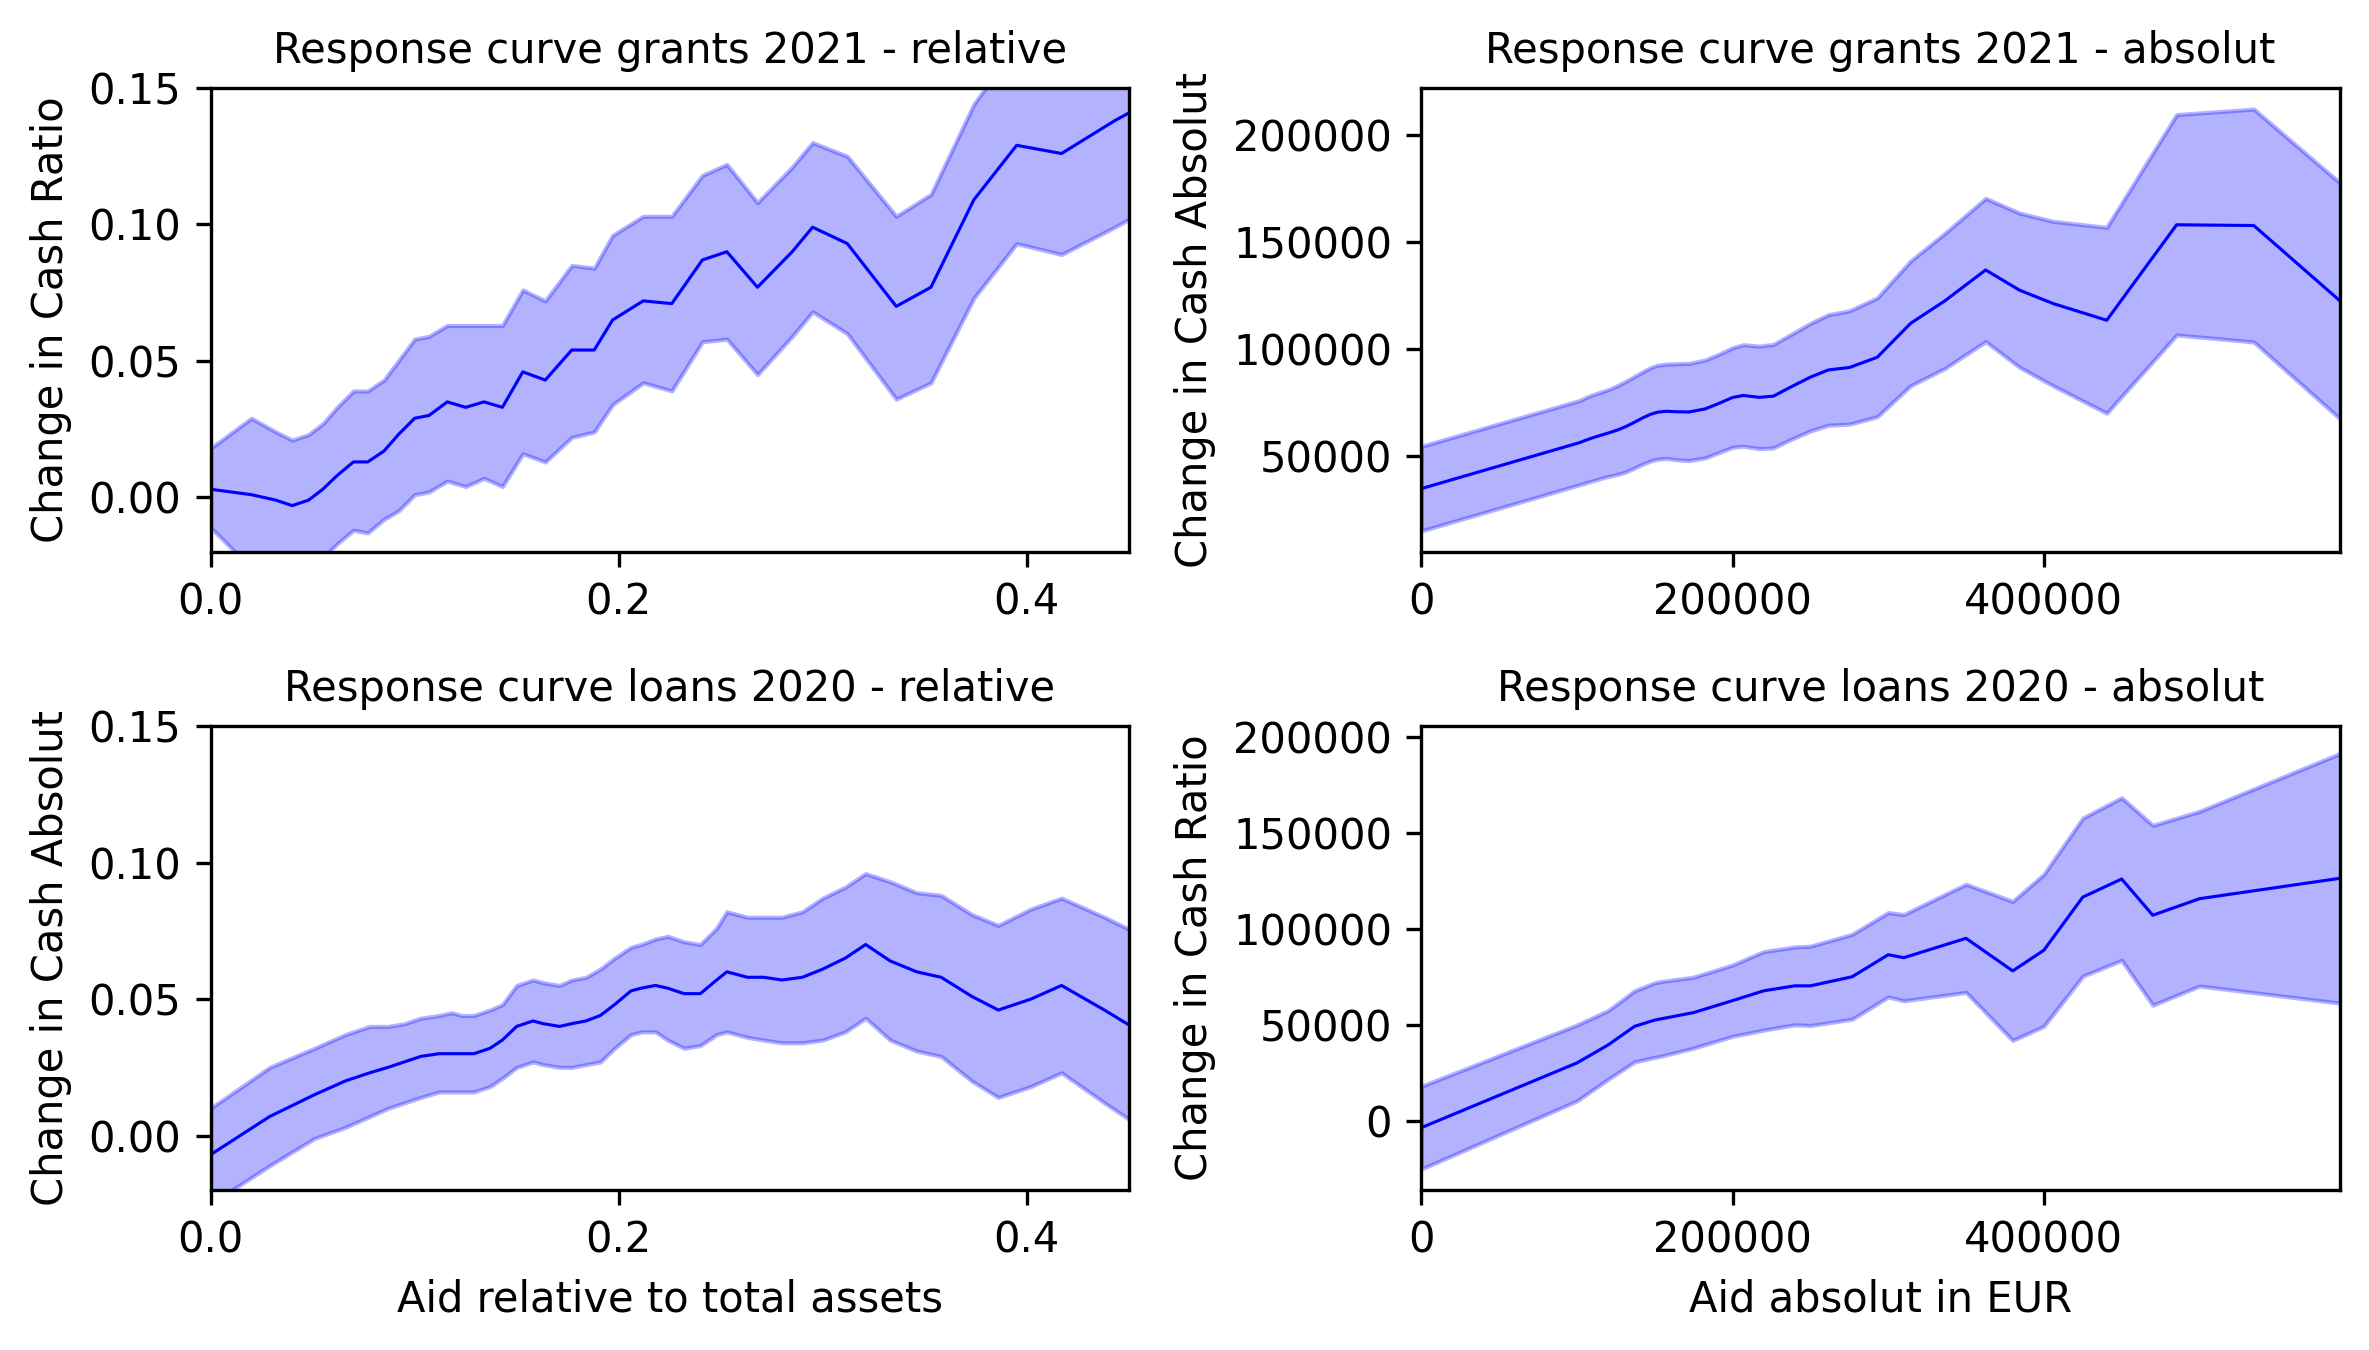
\includegraphics[width=1\columnwidth]{Figures/causal_curves1}}
    
    \decoRule
    \caption[Response curves for grants and loans]{Estimated Dose Response Functions, for liquidity (cash) from grants 2021 (top) and loans 2020 (bottom) in relative (left) and absolte (right) terms with 95\% Confidence Bands. For Binomial Distributed Data. The estimate of absolute variants used a lognormal GLM for the GPS estimation due to the different distribution of the variables.}
    \label{fig:Curve1}
\end{figure}


\subsection{The relationship of solvency and aid}


Figure \ref{fig:Curve2} shows the estimated dose response curves for loans and grants in 2021 with their effect on the indebtedness represented by the debt-to-asset ratio.
The downward trend on the left side indicated a negative effect on the debt ratio like the DiD estimates (- 0.03 \%) and an opposing trend in the respective relationship of loans, which confirms the initial assumption on the solvency effects.




\begin{figure}
    \centering
    \makebox[\textwidth][c]{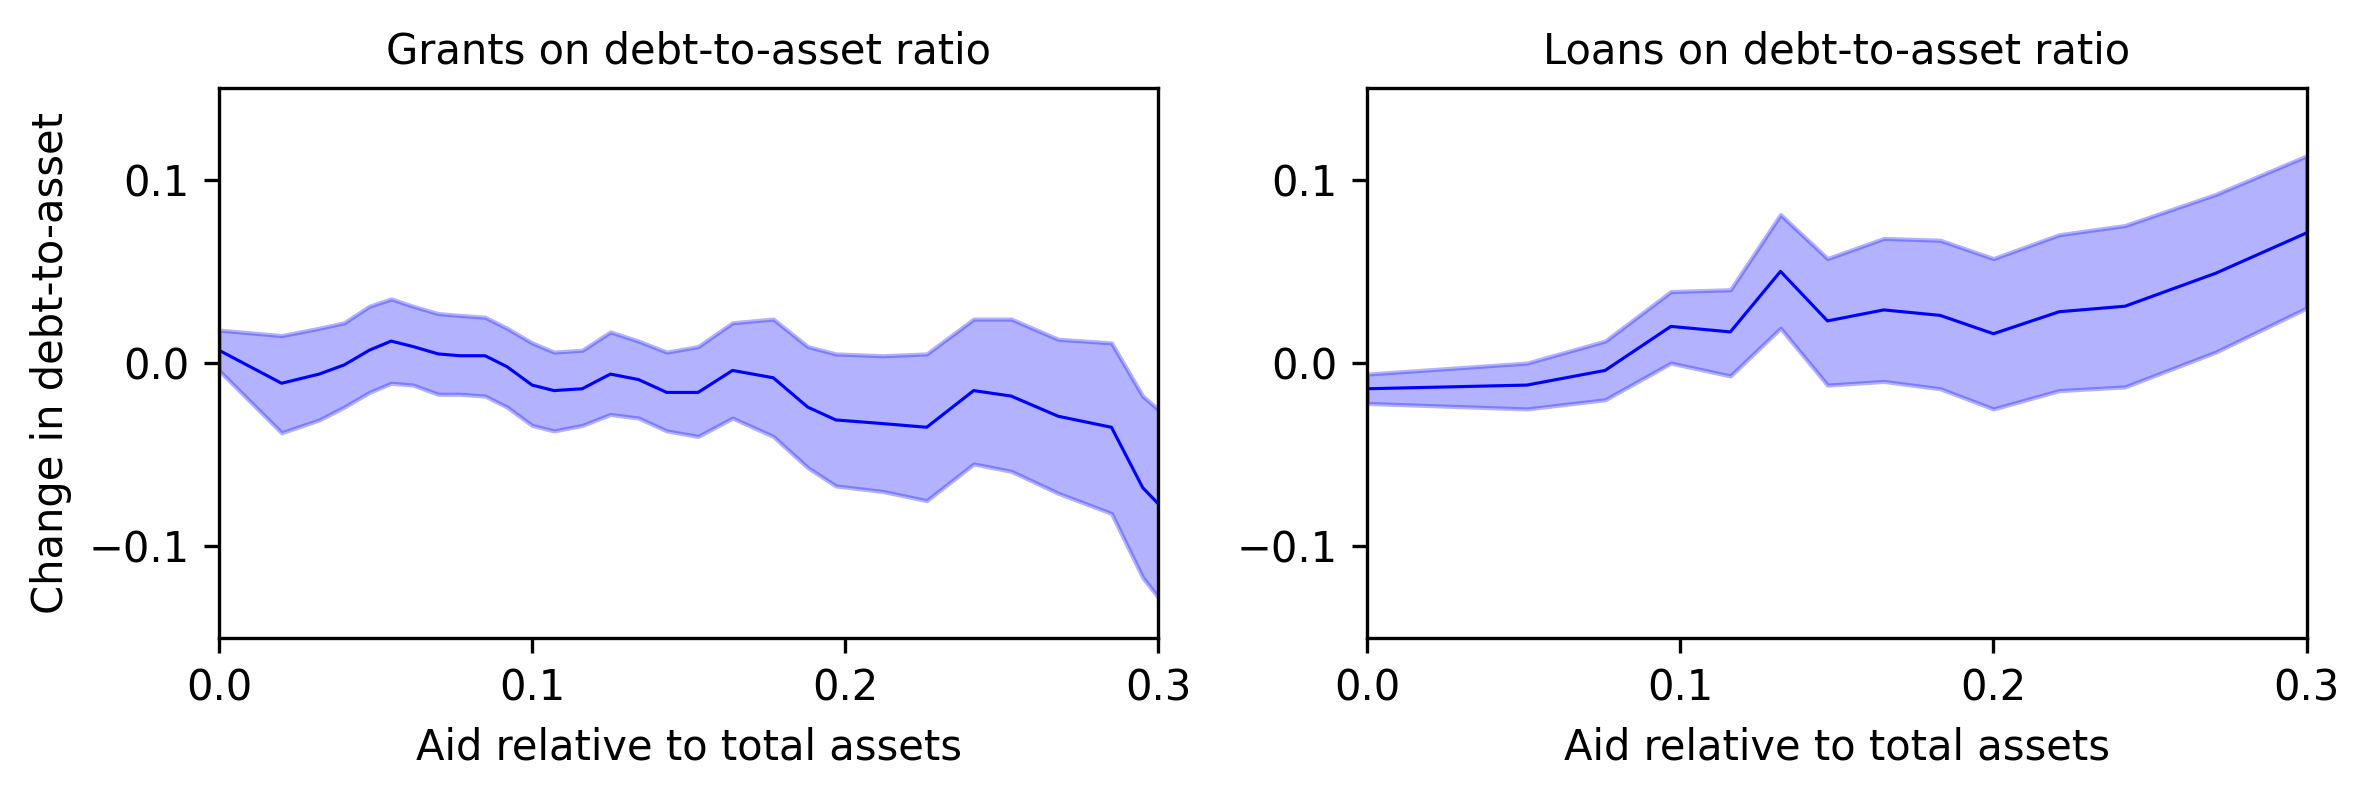
\includegraphics[width=1\columnwidth]{Figures/causal_curves2.png}}
    
    \decoRule
    \caption[Response curves for indebtedness through aid]{Estimated Dose Response Functions, for the debt-to-asset ratio from grants 2021 and loans 2021 in relative terms with 95\% Confidence Bands}
    \label{fig:Curve2}
\end{figure}


Figure \ref{fig:Curve3} show response curves for four selected industries that were used as example cases by \parencite{bischof_bedeutung_2021} for their assumption of heterogenous effects of grants between industries with different cost structures.


Of the four shows relations, the food and beverage sector has the highest transmission according to \parencite{bischof_bedeutung_2021}, followed by the travel agency and tour operator sector and then the creative, arts, and entertainment industry. Last, with the lowest factor is the industry of sports activities, amusement, and recreation.

With the estimated curves in Figure \ref{fig:Curve3}, the food and beverage sector has the most narrow confidence bands and the clearest upwards trends, while the least positive effect on the cash ratio can be interpreted for the travel agency and tour operator sector. However, the curves are highly sensitive to specifications and the wavy and wide confidence bands are indicating limited statistical significance and thus do not allow a reliable judgment confirming or denying a connection between the observed effects and the transmission factors from \parencite{bischof_bedeutung_2021}. 

Considering the additional industry curves from Figure \ref{fig:Curve4} in Appendix 1, it can only be cautiously conclude that the general assumption of heterogeneous effects between industries cannot be rejected with the results obtained.




\begin{figure}
    \centering
    \makebox[\textwidth][c]{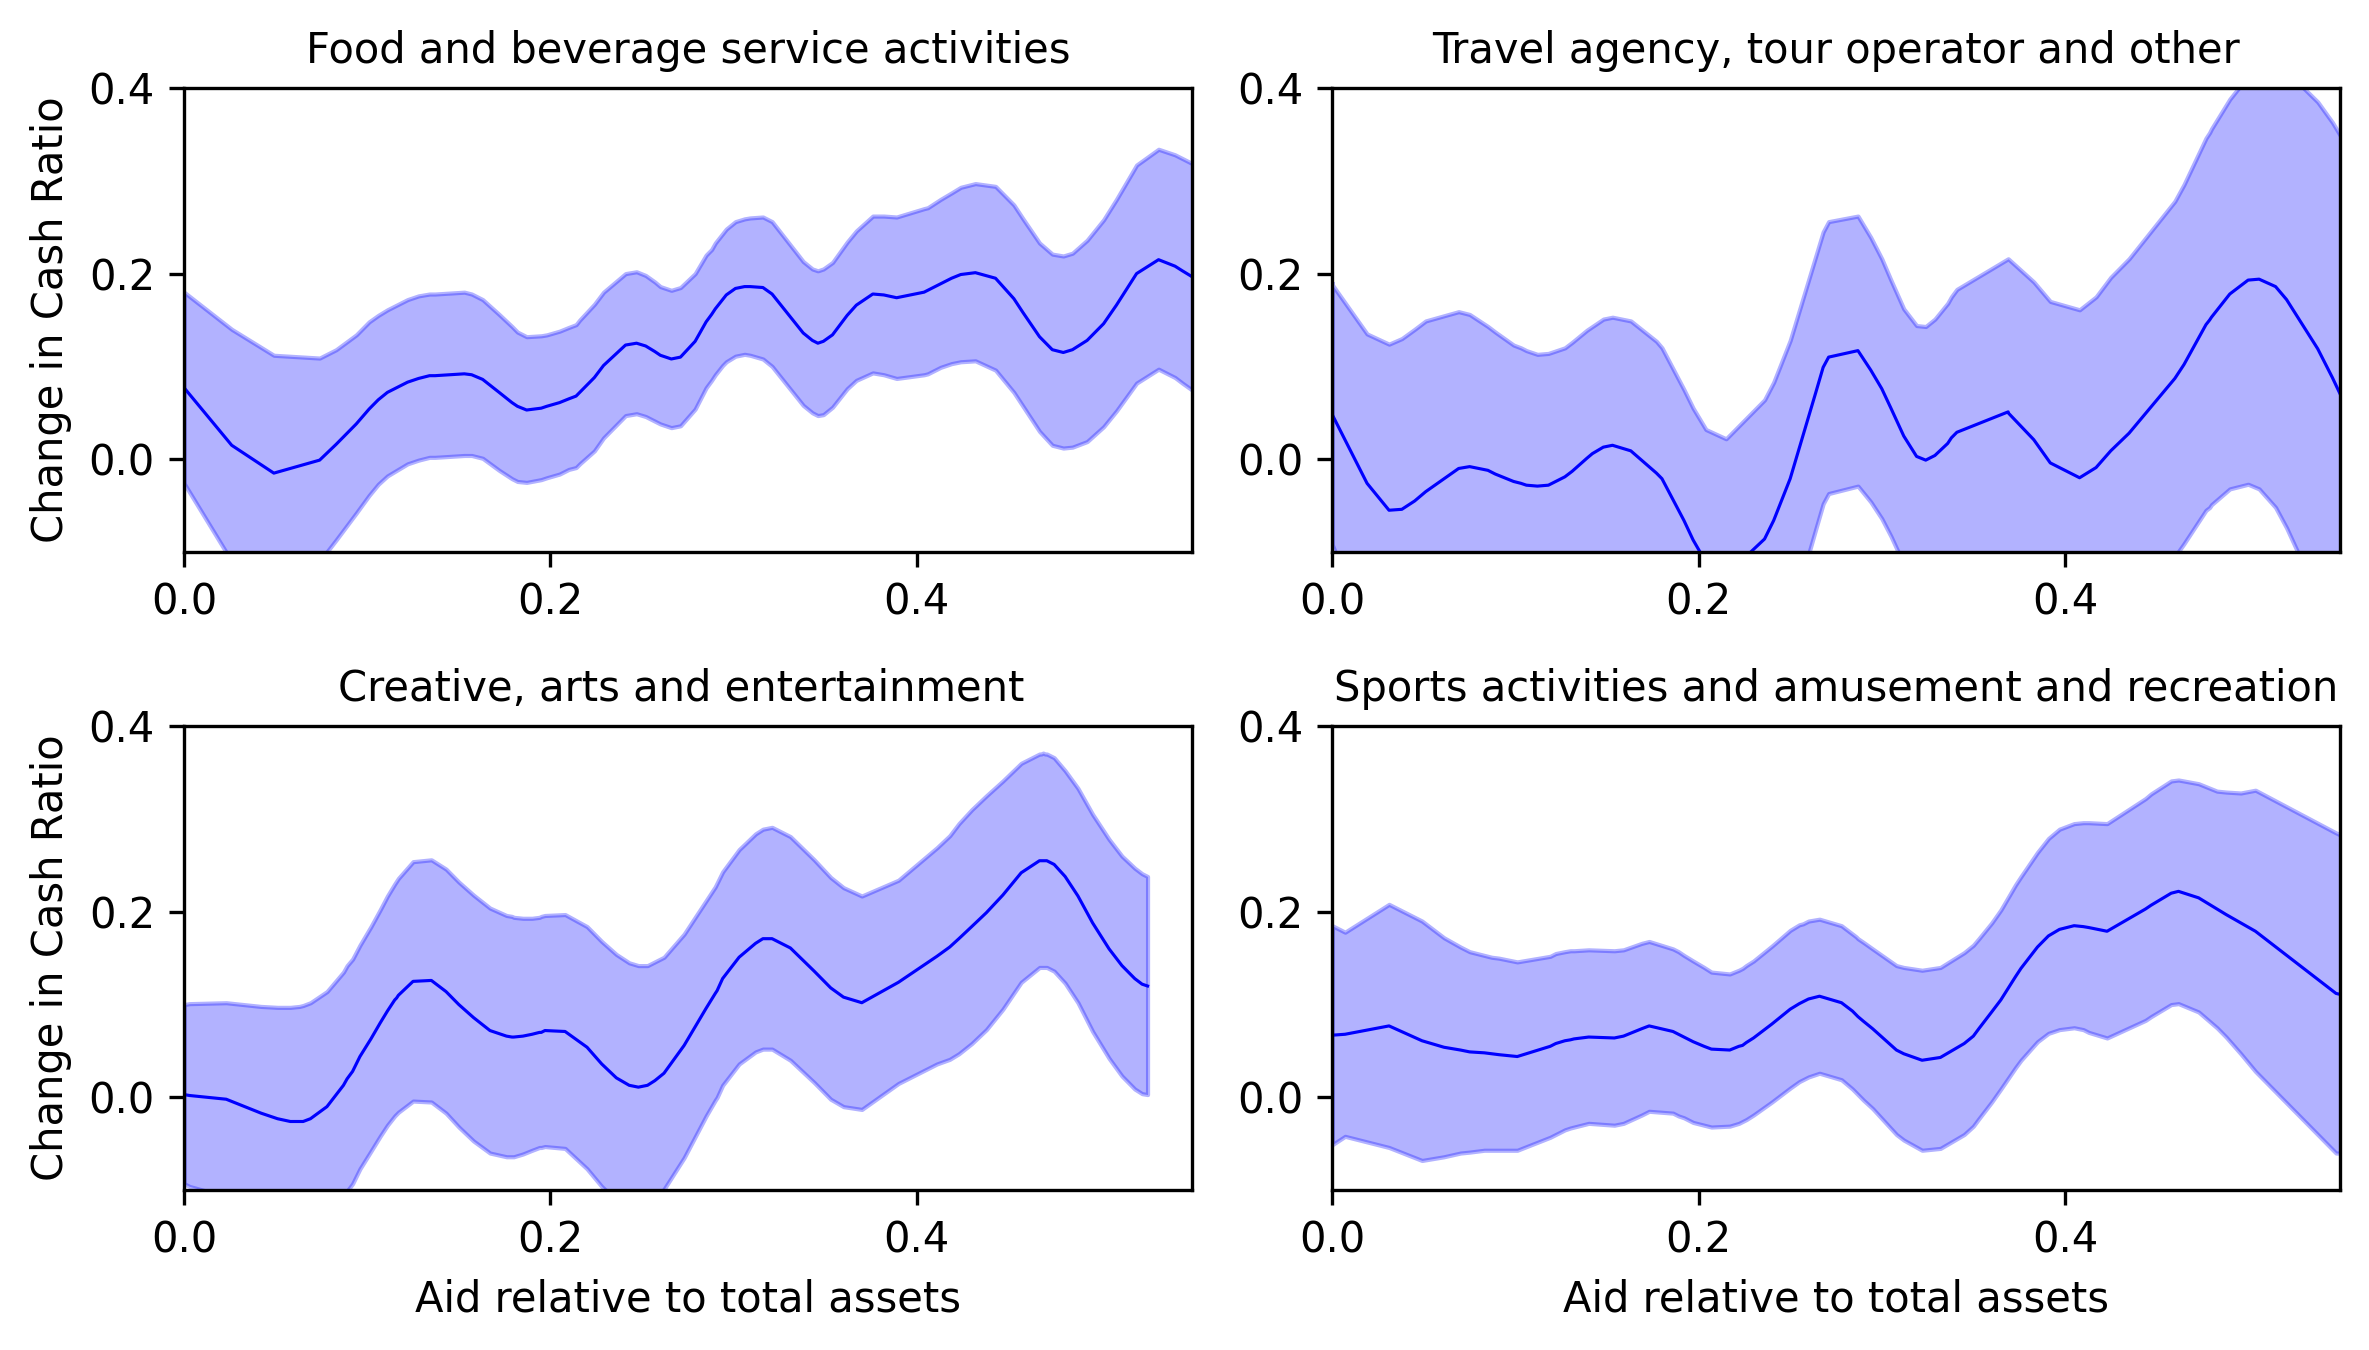
\includegraphics[width=1\columnwidth]{Figures/causal_curves_industries1.png}}
    
    \decoRule
    \caption[Response curves for liquidity through aid - by sectors 1]{Estimated Dose Response Functions, for the cash ratio from grants 2021 in selected industries in relative terms with 95\% Confidence Bands}
    \label{fig:Curve3}
\end{figure}



% Chapter Template

\chapter{Conclusion} % Main chapter title

\label{Chapter6} % Change X to a consecutive number; for referencing this chapter elsewhere, use \ref{ChapterX}

%----------------------------------------------------------------------------------------
%	SECTION 1
%----------------------------------------------------------------------------------------

\section{Policy Implications}





%----------------------------------------------------------------------------------------
%	SECTION 2
%----------------------------------------------------------------------------------------

\section{Conclusion}



%% Chapter 1

\chapter{Chapter Title Here} % Main chapter title

\label{Chapter1} % For referencing the chapter elsewhere, use \ref{Chapter1} 

%----------------------------------------------------------------------------------------

% Define some commands to keep the formatting separated from the content 
\newcommand{\keyword}[1]{\textbf{#1}}
\newcommand{\tabhead}[1]{\textbf{#1}}
\newcommand{\code}[1]{\texttt{#1}}
\newcommand{\file}[1]{\texttt{\bfseries#1}}
\newcommand{\option}[1]{\texttt{\itshape#1}}

%----------------------------------------------------------------------------------------

\section{Welcome and Thank You}
Welcome to this \LaTeX{} Thesis Template, a beautiful and easy to use template for writing a thesis using the \LaTeX{} typesetting system.

If you are writing a thesis (or will be in the future) and its subject is technical or mathematical (though it doesn't have to be), then creating it in \LaTeX{} is highly recommended as a way to make sure you can just get down to the essential writing without having to worry over formatting or wasting time arguing with your word processor.

\LaTeX{} is easily able to professionally typeset documents that run to hundreds or thousands of pages long. With simple mark-up commands, it automatically sets out the table of contents, margins, page headers and footers and keeps the formatting consistent and beautiful. One of its main strengths is the way it can easily typeset mathematics, even \emph{heavy} mathematics. Even if those equations are the most horribly twisted and most difficult mathematical problems that can only be solved on a super-computer, you can at least count on \LaTeX{} to make them look stunning.

%----------------------------------------------------------------------------------------

\section{Learning \LaTeX{}}

\LaTeX{} is not a \textsc{wysiwyg} (What You See is What You Get) program, unlike word processors such as Microsoft Word or Apple's Pages. Instead, a document written for \LaTeX{} is actually a simple, plain text file that contains \emph{no formatting}. You tell \LaTeX{} how you want the formatting in the finished document by writing in simple commands amongst the text, for example, if I want to use \emph{italic text for emphasis}, I write the \verb|\emph{text}| command and put the text I want in italics in between the curly braces. This means that \LaTeX{} is a \enquote{mark-up} language, very much like HTML.

\subsection{A (not so short) Introduction to \LaTeX{}}

If you are new to \LaTeX{}, there is a very good eBook -- freely available online as a PDF file -- called, \enquote{The Not So Short Introduction to \LaTeX{}}. The book's title is typically shortened to just \emph{lshort}. You can download the latest version (as it is occasionally updated) from here:
\url{http://www.ctan.org/tex-archive/info/lshort/english/lshort.pdf}

It is also available in several other languages. Find yours from the list on this page: \url{http://www.ctan.org/tex-archive/info/lshort/}

It is recommended to take a little time out to learn how to use \LaTeX{} by creating several, small `test' documents, or having a close look at several templates on:\\ 
\url{http://www.LaTeXTemplates.com}\\ 
Making the effort now means you're not stuck learning the system when what you \emph{really} need to be doing is writing your thesis.

\subsection{A Short Math Guide for \LaTeX{}}

If you are writing a technical or mathematical thesis, then you may want to read the document by the AMS (American Mathematical Society) called, \enquote{A Short Math Guide for \LaTeX{}}. It can be found online here:
\url{http://www.ams.org/tex/amslatex.html}
under the \enquote{Additional Documentation} section towards the bottom of the page.

\subsection{Common \LaTeX{} Math Symbols}
There are a multitude of mathematical symbols available for \LaTeX{} and it would take a great effort to learn the commands for them all. The most common ones you are likely to use are shown on this page:
\url{http://www.sunilpatel.co.uk/latex-type/latex-math-symbols/}

You can use this page as a reference or crib sheet, the symbols are rendered as large, high quality images so you can quickly find the \LaTeX{} command for the symbol you need.

\subsection{\LaTeX{} on a Mac}
 
The \LaTeX{} distribution is available for many systems including Windows, Linux and Mac OS X. The package for OS X is called MacTeX and it contains all the applications you need -- bundled together and pre-customized -- for a fully working \LaTeX{} environment and work flow.
 
MacTeX includes a custom dedicated \LaTeX{} editor called TeXShop for writing your `\file{.tex}' files and BibDesk: a program to manage your references and create your bibliography section just as easily as managing songs and creating playlists in iTunes.

%----------------------------------------------------------------------------------------

\section{Getting Started with this Template}

If you are familiar with \LaTeX{}, then you should explore the directory structure of the template and then proceed to place your own information into the \emph{THESIS INFORMATION} block of the \file{main.tex} file. You can then modify the rest of this file to your unique specifications based on your degree/university. Section \ref{FillingFile} on page \pageref{FillingFile} will help you do this. Make sure you also read section \ref{ThesisConventions} about thesis conventions to get the most out of this template.

If you are new to \LaTeX{} it is recommended that you carry on reading through the rest of the information in this document.

Before you begin using this template you should ensure that its style complies with the thesis style guidelines imposed by your institution. In most cases this template style and layout will be suitable. If it is not, it may only require a small change to bring the template in line with your institution's recommendations. These modifications will need to be done on the \file{MastersDoctoralThesis.cls} file.

\subsection{About this Template}

This \LaTeX{} Thesis Template is originally based and created around a \LaTeX{} style file created by Steve R.\ Gunn from the University of Southampton (UK), department of Electronics and Computer Science. You can find his original thesis style file at his site, here:
\url{http://www.ecs.soton.ac.uk/~srg/softwaretools/document/templates/}

Steve's \file{ecsthesis.cls} was then taken by Sunil Patel who modified it by creating a skeleton framework and folder structure to place the thesis files in. The resulting template can be found on Sunil's site here:
\url{http://www.sunilpatel.co.uk/thesis-template}

Sunil's template was made available through \url{http://www.LaTeXTemplates.com} where it was modified many times based on user requests and questions. Version 2.0 and onwards of this template represents a major modification to Sunil's template and is, in fact, hardly recognisable. The work to make version 2.0 possible was carried out by \href{mailto:vel@latextemplates.com}{Vel} and Johannes Böttcher.

%----------------------------------------------------------------------------------------

\section{What this Template Includes}

\subsection{Folders}

This template comes as a single zip file that expands out to several files and folders. The folder names are mostly self-explanatory:

\keyword{Appendices} -- this is the folder where you put the appendices. Each appendix should go into its own separate \file{.tex} file. An example and template are included in the directory.

\keyword{Chapters} -- this is the folder where you put the thesis chapters. A thesis usually has about six chapters, though there is no hard rule on this. Each chapter should go in its own separate \file{.tex} file and they can be split as:
\begin{itemize}
\item Chapter 1: Introduction to the thesis topic
\item Chapter 2: Background information and theory
\item Chapter 3: (Laboratory) experimental setup
\item Chapter 4: Details of experiment 1
\item Chapter 5: Details of experiment 2
\item Chapter 6: Discussion of the experimental results
\item Chapter 7: Conclusion and future directions
\end{itemize}
This chapter layout is specialised for the experimental sciences, your discipline may be different.

\keyword{Figures} -- this folder contains all figures for the thesis. These are the final images that will go into the thesis document.

\subsection{Files}

Included are also several files, most of them are plain text and you can see their contents in a text editor. After initial compilation, you will see that more auxiliary files are created by \LaTeX{} or BibTeX and which you don't need to delete or worry about:

\keyword{example.bib} -- this is an important file that contains all the bibliographic information and references that you will be citing in the thesis for use with BibTeX. You can write it manually, but there are reference manager programs available that will create and manage it for you. Bibliographies in \LaTeX{} are a large subject and you may need to read about BibTeX before starting with this. Many modern reference managers will allow you to export your references in BibTeX format which greatly eases the amount of work you have to do.

\keyword{MastersDoctoralThesis.cls} -- this is an important file. It is the class file that tells \LaTeX{} how to format the thesis. 

\keyword{main.pdf} -- this is your beautifully typeset thesis (in the PDF file format) created by \LaTeX{}. It is supplied in the PDF with the template and after you compile the template you should get an identical version.

\keyword{main.tex} -- this is an important file. This is the file that you tell \LaTeX{} to compile to produce your thesis as a PDF file. It contains the framework and constructs that tell \LaTeX{} how to layout the thesis. It is heavily commented so you can read exactly what each line of code does and why it is there. After you put your own information into the \emph{THESIS INFORMATION} block -- you have now started your thesis!

Files that are \emph{not} included, but are created by \LaTeX{} as auxiliary files include:

\keyword{main.aux} -- this is an auxiliary file generated by \LaTeX{}, if it is deleted \LaTeX{} simply regenerates it when you run the main \file{.tex} file.

\keyword{main.bbl} -- this is an auxiliary file generated by BibTeX, if it is deleted, BibTeX simply regenerates it when you run the \file{main.aux} file. Whereas the \file{.bib} file contains all the references you have, this \file{.bbl} file contains the references you have actually cited in the thesis and is used to build the bibliography section of the thesis.

\keyword{main.blg} -- this is an auxiliary file generated by BibTeX, if it is deleted BibTeX simply regenerates it when you run the main \file{.aux} file.

\keyword{main.lof} -- this is an auxiliary file generated by \LaTeX{}, if it is deleted \LaTeX{} simply regenerates it when you run the main \file{.tex} file. It tells \LaTeX{} how to build the \emph{List of Figures} section.

\keyword{main.log} -- this is an auxiliary file generated by \LaTeX{}, if it is deleted \LaTeX{} simply regenerates it when you run the main \file{.tex} file. It contains messages from \LaTeX{}, if you receive errors and warnings from \LaTeX{}, they will be in this \file{.log} file.

\keyword{main.lot} -- this is an auxiliary file generated by \LaTeX{}, if it is deleted \LaTeX{} simply regenerates it when you run the main \file{.tex} file. It tells \LaTeX{} how to build the \emph{List of Tables} section.

\keyword{main.out} -- this is an auxiliary file generated by \LaTeX{}, if it is deleted \LaTeX{} simply regenerates it when you run the main \file{.tex} file.

So from this long list, only the files with the \file{.bib}, \file{.cls} and \file{.tex} extensions are the most important ones. The other auxiliary files can be ignored or deleted as \LaTeX{} and BibTeX will regenerate them.

%----------------------------------------------------------------------------------------

\section{Filling in Your Information in the \file{main.tex} File}\label{FillingFile}

You will need to personalise the thesis template and make it your own by filling in your own information. This is done by editing the \file{main.tex} file in a text editor or your favourite LaTeX environment.

Open the file and scroll down to the third large block titled \emph{THESIS INFORMATION} where you can see the entries for \emph{University Name}, \emph{Department Name}, etc \ldots

Fill out the information about yourself, your group and institution. You can also insert web links, if you do, make sure you use the full URL, including the \code{http://} for this. If you don't want these to be linked, simply remove the \verb|\href{url}{name}| and only leave the name.

When you have done this, save the file and recompile \code{main.tex}. All the information you filled in should now be in the PDF, complete with web links. You can now begin your thesis proper!

%----------------------------------------------------------------------------------------

\section{The \code{main.tex} File Explained}

The \file{main.tex} file contains the structure of the thesis. There are plenty of written comments that explain what pages, sections and formatting the \LaTeX{} code is creating. Each major document element is divided into commented blocks with titles in all capitals to make it obvious what the following bit of code is doing. Initially there seems to be a lot of \LaTeX{} code, but this is all formatting, and it has all been taken care of so you don't have to do it.

Begin by checking that your information on the title page is correct. For the thesis declaration, your institution may insist on something different than the text given. If this is the case, just replace what you see with what is required in the \emph{DECLARATION PAGE} block.

Then comes a page which contains a funny quote. You can put your own, or quote your favourite scientist, author, person, and so on. Make sure to put the name of the person who you took the quote from.

Following this is the abstract page which summarises your work in a condensed way and can almost be used as a standalone document to describe what you have done. The text you write will cause the heading to move up so don't worry about running out of space.

Next come the acknowledgements. On this page, write about all the people who you wish to thank (not forgetting parents, partners and your advisor/supervisor).

The contents pages, list of figures and tables are all taken care of for you and do not need to be manually created or edited. The next set of pages are more likely to be optional and can be deleted since they are for a more technical thesis: insert a list of abbreviations you have used in the thesis, then a list of the physical constants and numbers you refer to and finally, a list of mathematical symbols used in any formulae. Making the effort to fill these tables means the reader has a one-stop place to refer to instead of searching the internet and references to try and find out what you meant by certain abbreviations or symbols.

The list of symbols is split into the Roman and Greek alphabets. Whereas the abbreviations and symbols ought to be listed in alphabetical order (and this is \emph{not} done automatically for you) the list of physical constants should be grouped into similar themes.

The next page contains a one line dedication. Who will you dedicate your thesis to?

Finally, there is the block where the chapters are included. Uncomment the lines (delete the \code{\%} character) as you write the chapters. Each chapter should be written in its own file and put into the \emph{Chapters} folder and named \file{Chapter1}, \file{Chapter2}, etc\ldots Similarly for the appendices, uncomment the lines as you need them. Each appendix should go into its own file and placed in the \emph{Appendices} folder.

After the preamble, chapters and appendices finally comes the bibliography. The bibliography style (called \option{authoryear}) is used for the bibliography and is a fully featured style that will even include links to where the referenced paper can be found online. Do not underestimate how grateful your reader will be to find that a reference to a paper is just a click away. Of course, this relies on you putting the URL information into the BibTeX file in the first place.

%----------------------------------------------------------------------------------------

\section{Thesis Features and Conventions}\label{ThesisConventions}

To get the best out of this template, there are a few conventions that you may want to follow.

One of the most important (and most difficult) things to keep track of in such a long document as a thesis is consistency. Using certain conventions and ways of doing things (such as using a Todo list) makes the job easier. Of course, all of these are optional and you can adopt your own method.

\subsection{Printing Format}

This thesis template is designed for double sided printing (i.e. content on the front and back of pages) as most theses are printed and bound this way. Switching to one sided printing is as simple as uncommenting the \option{oneside} option of the \code{documentclass} command at the top of the \file{main.tex} file. You may then wish to adjust the margins to suit specifications from your institution.

The headers for the pages contain the page number on the outer side (so it is easy to flick through to the page you want) and the chapter name on the inner side.

The text is set to 11 point by default with single line spacing, again, you can tune the text size and spacing should you want or need to using the options at the very start of \file{main.tex}. The spacing can be changed similarly by replacing the \option{singlespacing} with \option{onehalfspacing} or \option{doublespacing}.

\subsection{Using US Letter Paper}

The paper size used in the template is A4, which is the standard size in Europe. If you are using this thesis template elsewhere and particularly in the United States, then you may have to change the A4 paper size to the US Letter size. This can be done in the margins settings section in \file{main.tex}.

Due to the differences in the paper size, the resulting margins may be different to what you like or require (as it is common for institutions to dictate certain margin sizes). If this is the case, then the margin sizes can be tweaked by modifying the values in the same block as where you set the paper size. Now your document should be set up for US Letter paper size with suitable margins.

\subsection{References}

The \code{biblatex} package is used to format the bibliography and inserts references such as this one \parencite{Reference1}. The options used in the \file{main.tex} file mean that the in-text citations of references are formatted with the author(s) listed with the date of the publication. Multiple references are separated by semicolons (e.g. \parencite{Reference2, Reference1}) and references with more than three authors only show the first author with \emph{et al.} indicating there are more authors (e.g. \parencite{Reference3}). This is done automatically for you. To see how you use references, have a look at the \file{Chapter1.tex} source file. Many reference managers allow you to simply drag the reference into the document as you type.

Scientific references should come \emph{before} the punctuation mark if there is one (such as a comma or period). The same goes for footnotes\footnote{Such as this footnote, here down at the bottom of the page.}. You can change this but the most important thing is to keep the convention consistent throughout the thesis. Footnotes themselves should be full, descriptive sentences (beginning with a capital letter and ending with a full stop). The APA6 states: \enquote{Footnote numbers should be superscripted, [...], following any punctuation mark except a dash.} The Chicago manual of style states: \enquote{A note number should be placed at the end of a sentence or clause. The number follows any punctuation mark except the dash, which it precedes. It follows a closing parenthesis.}

The bibliography is typeset with references listed in alphabetical order by the first author's last name. This is similar to the APA referencing style. To see how \LaTeX{} typesets the bibliography, have a look at the very end of this document (or just click on the reference number links in in-text citations).

\subsubsection{A Note on bibtex}

The bibtex backend used in the template by default does not correctly handle unicode character encoding (i.e. "international" characters). You may see a warning about this in the compilation log and, if your references contain unicode characters, they may not show up correctly or at all. The solution to this is to use the biber backend instead of the outdated bibtex backend. This is done by finding this in \file{main.tex}: \option{backend=bibtex} and changing it to \option{backend=biber}. You will then need to delete all auxiliary BibTeX files and navigate to the template directory in your terminal (command prompt). Once there, simply type \code{biber main} and biber will compile your bibliography. You can then compile \file{main.tex} as normal and your bibliography will be updated. An alternative is to set up your LaTeX editor to compile with biber instead of bibtex, see \href{http://tex.stackexchange.com/questions/154751/biblatex-with-biber-configuring-my-editor-to-avoid-undefined-citations/}{here} for how to do this for various editors.

\subsection{Tables}

Tables are an important way of displaying your results, below is an example table which was generated with this code:

{\small
\begin{verbatim}
\begin{table}
\caption{The effects of treatments X and Y on the four groups studied.}
\label{tab:treatments}
\centering
\begin{tabular}{l l l}
\toprule
\tabhead{Groups} & \tabhead{Treatment X} & \tabhead{Treatment Y} \\
\midrule
1 & 0.2 & 0.8\\
2 & 0.17 & 0.7\\
3 & 0.24 & 0.75\\
4 & 0.68 & 0.3\\
\bottomrule\\
\end{tabular}
\end{table}
\end{verbatim}
}

\begin{table}
\caption{The effects of treatments X and Y on the four groups studied.}
\label{tab:treatments}
\centering
\begin{tabular}{l l l}
\toprule
\tabhead{Groups} & \tabhead{Treatment X} & \tabhead{Treatment Y} \\
\midrule
1 & 0.2 & 0.8\\
2 & 0.17 & 0.7\\
3 & 0.24 & 0.75\\
4 & 0.68 & 0.3\\
\bottomrule\\
\end{tabular}
\end{table}

You can reference tables with \verb|\ref{<label>}| where the label is defined within the table environment. See \file{Chapter1.tex} for an example of the label and citation (e.g. Table~\ref{tab:treatments}).

\subsection{Figures}

There will hopefully be many figures in your thesis (that should be placed in the \emph{Figures} folder). The way to insert figures into your thesis is to use a code template like this:
\begin{verbatim}
\begin{figure}
\centering

\includegraphics{Figures/Electron}
\decoRule
\caption[An Electron]{An electron (artist's impression).}
\label{fig:Electron}
\end{figure}
\end{verbatim}
Also look in the source file. Putting this code into the source file produces the picture of the electron that you can see in the figure below.

\begin{figure}[th]
\centering

\includegraphics{Figures/Electron}
\decoRule
\caption[An Electron]{An electron (artist's impression).}
\label{fig:Electron}
\end{figure}

Sometimes figures don't always appear where you write them in the source. The placement depends on how much space there is on the page for the figure. Sometimes there is not enough room to fit a figure directly where it should go (in relation to the text) and so \LaTeX{} puts it at the top of the next page. Positioning figures is the job of \LaTeX{} and so you should only worry about making them look good!

Figures usually should have captions just in case you need to refer to them (such as in Figure~\ref{fig:Electron}). The \verb|\caption| command contains two parts, the first part, inside the square brackets is the title that will appear in the \emph{List of Figures}, and so should be short. The second part in the curly brackets should contain the longer and more descriptive caption text.

The \verb|\decoRule| command is optional and simply puts an aesthetic horizontal line below the image. If you do this for one image, do it for all of them.

\LaTeX{} is capable of using images in pdf, jpg and png format.

\subsection{Typesetting mathematics}

If your thesis is going to contain heavy mathematical content, be sure that \LaTeX{} will make it look beautiful, even though it won't be able to solve the equations for you.

The \enquote{Not So Short Introduction to \LaTeX} (available on \href{http://www.ctan.org/tex-archive/info/lshort/english/lshort.pdf}{CTAN}) should tell you everything you need to know for most cases of typesetting mathematics. If you need more information, a much more thorough mathematical guide is available from the AMS called, \enquote{A Short Math Guide to \LaTeX} and can be downloaded from:
\url{ftp://ftp.ams.org/pub/tex/doc/amsmath/short-math-guide.pdf}

There are many different \LaTeX{} symbols to remember, luckily you can find the most common symbols in \href{http://ctan.org/pkg/comprehensive}{The Comprehensive \LaTeX~Symbol List}.

You can write an equation, which is automatically given an equation number by \LaTeX{} like this:
\begin{verbatim}
\begin{equation}
E = mc^{2}
\label{eqn:Einstein}
\end{equation}
\end{verbatim}

This will produce Einstein's famous energy-matter equivalence equation:
\begin{equation}
E = mc^{2}
\label{eqn:Einstein}
\end{equation}

All equations you write (which are not in the middle of paragraph text) are automatically given equation numbers by \LaTeX{}. If you don't want a particular equation numbered, use the unnumbered form:
\begin{verbatim}
\[ a^{2}=4 \]
\end{verbatim}

%----------------------------------------------------------------------------------------

\section{Sectioning and Subsectioning}

You should break your thesis up into nice, bite-sized sections and subsections. \LaTeX{} automatically builds a table of Contents by looking at all the \verb|\chapter{}|, \verb|\section{}|  and \verb|\subsection{}| commands you write in the source.

The Table of Contents should only list the sections to three (3) levels. A \verb|chapter{}| is level zero (0). A \verb|\section{}| is level one (1) and so a \verb|\subsection{}| is level two (2). In your thesis it is likely that you will even use a \verb|subsubsection{}|, which is level three (3). The depth to which the Table of Contents is formatted is set within \file{MastersDoctoralThesis.cls}. If you need this changed, you can do it in \file{main.tex}.

%----------------------------------------------------------------------------------------

\section{In Closing}

You have reached the end of this mini-guide. You can now rename or overwrite this pdf file and begin writing your own \file{Chapter1.tex} and the rest of your thesis. The easy work of setting up the structure and framework has been taken care of for you. It's now your job to fill it out!

Good luck and have lots of fun!

\begin{flushright}
Guide written by ---\\
Sunil Patel: \href{http://www.sunilpatel.co.uk}{www.sunilpatel.co.uk}\\
Vel: \href{http://www.LaTeXTemplates.com}{LaTeXTemplates.com}
\end{flushright}

%\include{Chapters/Chapter2} 
%\include{Chapters/Chapter3}
%\include{Chapters/Chapter4} 
%\include{Chapters/Chapter5} 

%----------------------------------------------------------------------------------------
%	THESIS CONTENT - APPENDICES
%----------------------------------------------------------------------------------------

\appendix % Cue to tell LaTeX that the following "chapters" are Appendices

% Include the appendices of the thesis as separate files from the Appendices folder
% Uncomment the lines as you write the Appendices

% Appendix A

\chapter{Frequently Asked Questions} % Main appendix title

\label{AppendixA} % For referencing this appendix elsewhere, use \ref{AppendixA}

\section{How do I change the colors of links?}

The color of links can be changed to your liking using:

{\small\verb!\hypersetup{urlcolor=red}!}, or

{\small\verb!\hypersetup{citecolor=green}!}, or

{\small\verb!\hypersetup{allcolor=blue}!}.

\noindent If you want to completely hide the links, you can use:

{\small\verb!\hypersetup{allcolors=.}!}, or even better: 

{\small\verb!\hypersetup{hidelinks}!}.

\noindent If you want to have obvious links in the PDF but not the printed text, use:

{\small\verb!\hypersetup{colorlinks=false}!}.


\begin{table}
    \caption{Complete coefficients for government aid impact on ratios}
    \label{tab:DiDresultsAll}
    \centering
    \def\arraystretch{1.2}
    \centering
    \begin{tabular}{llllll}
\toprule
     &      &                &                 aid &               post &            aid*post \\
type & year & ratio &                     &                    &                     \\
\midrule
grant & 2020 & cash &   0.0283*** (0.000) &    -0.0023 (0.322) &     -0.0089 (0.270) \\
     &      & quick &   0.2112*** (0.000) &   0.321*** (0.000) &     -0.0937 (0.221) \\
     &      & current &      0.0655 (0.274) &  0.3501*** (0.000) &     -0.0825 (0.330) \\
     &      & debt to equity &  -0.2703*** (0.009) &    -0.0676 (0.111) &     0.2478* (0.089) \\
     &      & equity &      0.0095 (0.268) &  0.0124*** (0.001) &     -0.0112 (0.371) \\
     &      & debt to assest &  -0.0347*** (0.001) &    -0.0047 (0.295) &   0.0412*** (0.006) \\
loan & 2020 & cash &  -0.0406*** (0.000) &    -0.0001 (0.966) &   0.0527*** (0.000) \\
     &      & quick &  -0.2065*** (0.000) &  0.2744*** (0.000) &   0.1085*** (0.000) \\
     &      & current &  -0.1688*** (0.000) &  0.3123*** (0.000) &   0.1271*** (0.000) \\
     &      & debt to equity &   0.3667*** (0.000) &     -0.055 (0.291) &   0.7306*** (0.000) \\
     &      & equity &    -0.0058* (0.069) &  0.0126*** (0.000) &  -0.0486*** (0.000) \\
     &      & debt to assest &   0.0398*** (0.000) &    -0.0013 (0.751) &   0.0715*** (0.000) \\
grant & 2021 & cash &   -0.0159** (0.033) &  -0.0199** (0.037) &   0.0768*** (0.000) \\
     &      & quick &   0.2879*** (0.002) &     0.0147 (0.899) &      0.0913 (0.478) \\
     &      & current &    0.2055** (0.039) &     0.0768 (0.544) &      0.0476 (0.736) \\
     &      & debt to equity &    -0.1569* (0.065) &     0.0167 (0.877) &     -0.1592 (0.185) \\
     &      & equity &      0.0123 (0.238) &        0.0 (0.998) &      0.0108 (0.465) \\
     &      & debt to assest &    -0.0231* (0.058) &     0.0135 (0.385) &    -0.0302* (0.079) \\
loan & 2021 & cash &  -0.0319*** (0.000) &  -0.0153** (0.027) &   0.0351*** (0.000) \\
     &      & quick &  -0.2017*** (0.000) &     0.0715 (0.269) &      0.0929 (0.252) \\
     &      & current &  -0.2285*** (0.001) &     0.1031 (0.188) &     0.1828* (0.064) \\
     &      & debt to equity &   0.4226*** (0.005) &     0.0749 (0.656) &    0.5043** (0.016) \\
     &      & equity &    -0.0159* (0.082) &    -0.0007 (0.947) &   -0.037*** (0.004) \\
     &      & debt to assest &   0.0379*** (0.001) &     0.0165 (0.219) &   0.0526*** (0.002) \\
\bottomrule
\end{tabular}
}

    \small  Notes: Standard errors in parentheses, *** p<0.01, ** p<0.05, * p<0.1

    \end{table}


% Appendix B

\chapter{Full list of insolvent aid  beneficiaries by industry} % Main appendix title

\label{AppendixB} % 

    \begin{table}
        \caption{Share of insolvent aid  beneficiaries by industry}
        \label{tab:InsByIndustry}
        \centering
        \def\arraystretch{1}
        \centering
        \begin{tabular}{lrrl}
\toprule
                                industry &  aid beneficiaries &  insolvent & share \\
\midrule
                   Employment activities &                594 &         30 & 5.05\% \\
               Construction of buildings &               1247 &         37 & 2.97\% \\
             Manufacture of basic metals &                586 &         14 & 2.39\% \\
Computer programming, consultancy and re &               1481 &         35 & 2.36\% \\
Manufacture of machinery and equipment n &               2226 &         44 & 1.98\% \\
Manufacture of computer, electronic and  &                728 &         13 & 1.79\% \\
     Specialised construction activities &               4103 &         68 & 1.66\% \\
Manufacture of rubber and plastic produc &                664 &         10 & 1.51\% \\
Printing and reproduction of recorded me &                826 &         11 & 1.33\% \\
                     Other manufacturing &                689 &          9 & 1.31\% \\
Architectural and engineering activities &                929 &         12 & 1.29\% \\
Manufacture of fabricated metal products &               3105 &         40 & 1.29\% \\
Land transport and transport via pipelin &               2552 &         31 & 1.21\% \\
            Manufacture of food products &               1537 &         17 & 1.11\% \\
         Gambling and betting activities &               2061 &         22 & 1.07\% \\
Wholesale trade, except of motor vehicle &               5396 &         56 & 1.04\% \\
       Other personal service activities &               2517 &         25 & 0.99\% \\
Services to buildings and landscape acti &               1018 &         10 & 0.98\% \\
Retail trade, except of motor vehicles a &               8810 &         84 & 0.95\% \\
Warehousing and support activities for t &               1620 &         15 & 0.93\% \\
Office administrative, office support an &               3040 &         28 & 0.92\% \\
         Advertising and market research &                952 &          8 & 0.84\% \\
                  Real estate activities &               1413 &         11 & 0.78\% \\
                Manufacture of furniture &                530 &          4 & 0.75\% \\
Activities of head offices; management c &                967 &          6 & 0.62\% \\
    Food and beverage service activities &              15173 &         88 & 0.58\% \\
           Rental and leasing activities &                868 &          5 & 0.58\% \\
Sports activities and amusement and recr &               5232 &         27 & 0.52\% \\
                               Education &                974 &          5 & 0.51\% \\
Wholesale and retail trade and repair of &               3525 &         17 & 0.48\% \\
Creative, arts and entertainment activit &               1485 &          6 & 0.40\% \\
                 Human health activities &               1417 &          5 & 0.35\% \\
Travel agency, tour operator and other r &               2756 &          8 & 0.29\% \\
Motion picture, video and television pro &                691 &          2 & 0.29\% \\
                           Accommodation &               9885 &         24 & 0.24\% \\
Crop and animal production, hunting and  &               1803 &          4 & 0.22\% \\
         Legal and accounting activities &                646 &          1 & 0.15\% \\
\bottomrule
\end{tabular}
}
    
        \small  Notes: Tables shows industries with more than 500 beneficiaries
    
        \end{table}
%% Appendix B
\chapter{Appendix B}
\label{AppendixB} % 
%\chapter{Full list of insolvent aid  beneficiaries by industry} % Main appendix title
\section{Full list of insolvent aid  beneficiaries by industry}


\begin{table}
        \caption{Share of insolvent aid  beneficiaries by industry}
        \label{tab:InsByIndustry}
        \centering
        \def\arraystretch{1}
        \centering
        \begin{tabular}{lrrl}
\toprule
                                industry &  aid beneficiaries &  insolvent & share \\
\midrule
                   Employment activities &                594 &         30 & 5.05\% \\
               Construction of buildings &               1247 &         37 & 2.97\% \\
             Manufacture of basic metals &                586 &         14 & 2.39\% \\
Computer programming, consultancy and re &               1481 &         35 & 2.36\% \\
Manufacture of machinery and equipment n &               2226 &         44 & 1.98\% \\
Manufacture of computer, electronic and  &                728 &         13 & 1.79\% \\
     Specialised construction activities &               4103 &         68 & 1.66\% \\
Manufacture of rubber and plastic produc &                664 &         10 & 1.51\% \\
Printing and reproduction of recorded me &                826 &         11 & 1.33\% \\
                     Other manufacturing &                689 &          9 & 1.31\% \\
Architectural and engineering activities &                929 &         12 & 1.29\% \\
Manufacture of fabricated metal products &               3105 &         40 & 1.29\% \\
Land transport and transport via pipelin &               2552 &         31 & 1.21\% \\
            Manufacture of food products &               1537 &         17 & 1.11\% \\
         Gambling and betting activities &               2061 &         22 & 1.07\% \\
Wholesale trade, except of motor vehicle &               5396 &         56 & 1.04\% \\
       Other personal service activities &               2517 &         25 & 0.99\% \\
Services to buildings and landscape acti &               1018 &         10 & 0.98\% \\
Retail trade, except of motor vehicles a &               8810 &         84 & 0.95\% \\
Warehousing and support activities for t &               1620 &         15 & 0.93\% \\
Office administrative, office support an &               3040 &         28 & 0.92\% \\
         Advertising and market research &                952 &          8 & 0.84\% \\
                  Real estate activities &               1413 &         11 & 0.78\% \\
                Manufacture of furniture &                530 &          4 & 0.75\% \\
Activities of head offices; management c &                967 &          6 & 0.62\% \\
    Food and beverage service activities &              15173 &         88 & 0.58\% \\
           Rental and leasing activities &                868 &          5 & 0.58\% \\
Sports activities and amusement and recr &               5232 &         27 & 0.52\% \\
                               Education &                974 &          5 & 0.51\% \\
Wholesale and retail trade and repair of &               3525 &         17 & 0.48\% \\
Creative, arts and entertainment activit &               1485 &          6 & 0.40\% \\
                 Human health activities &               1417 &          5 & 0.35\% \\
Travel agency, tour operator and other r &               2756 &          8 & 0.29\% \\
Motion picture, video and television pro &                691 &          2 & 0.29\% \\
                           Accommodation &               9885 &         24 & 0.24\% \\
Crop and animal production, hunting and  &               1803 &          4 & 0.22\% \\
         Legal and accounting activities &                646 &          1 & 0.15\% \\
\bottomrule
\end{tabular}
}
    
        \small  Notes: Tables shows industries with more than 500 beneficiaries
    
\end{table}

%
% Appendix C
\chapter{Appendix C}
%\chapter{Additional curves for selected industry } % Main appendix title


%\label{AppendixC} % 



% 1
\section{Figure 5.3 with full Axis range}

\begin{figure}
    \centering
    \makebox[\textwidth][c]{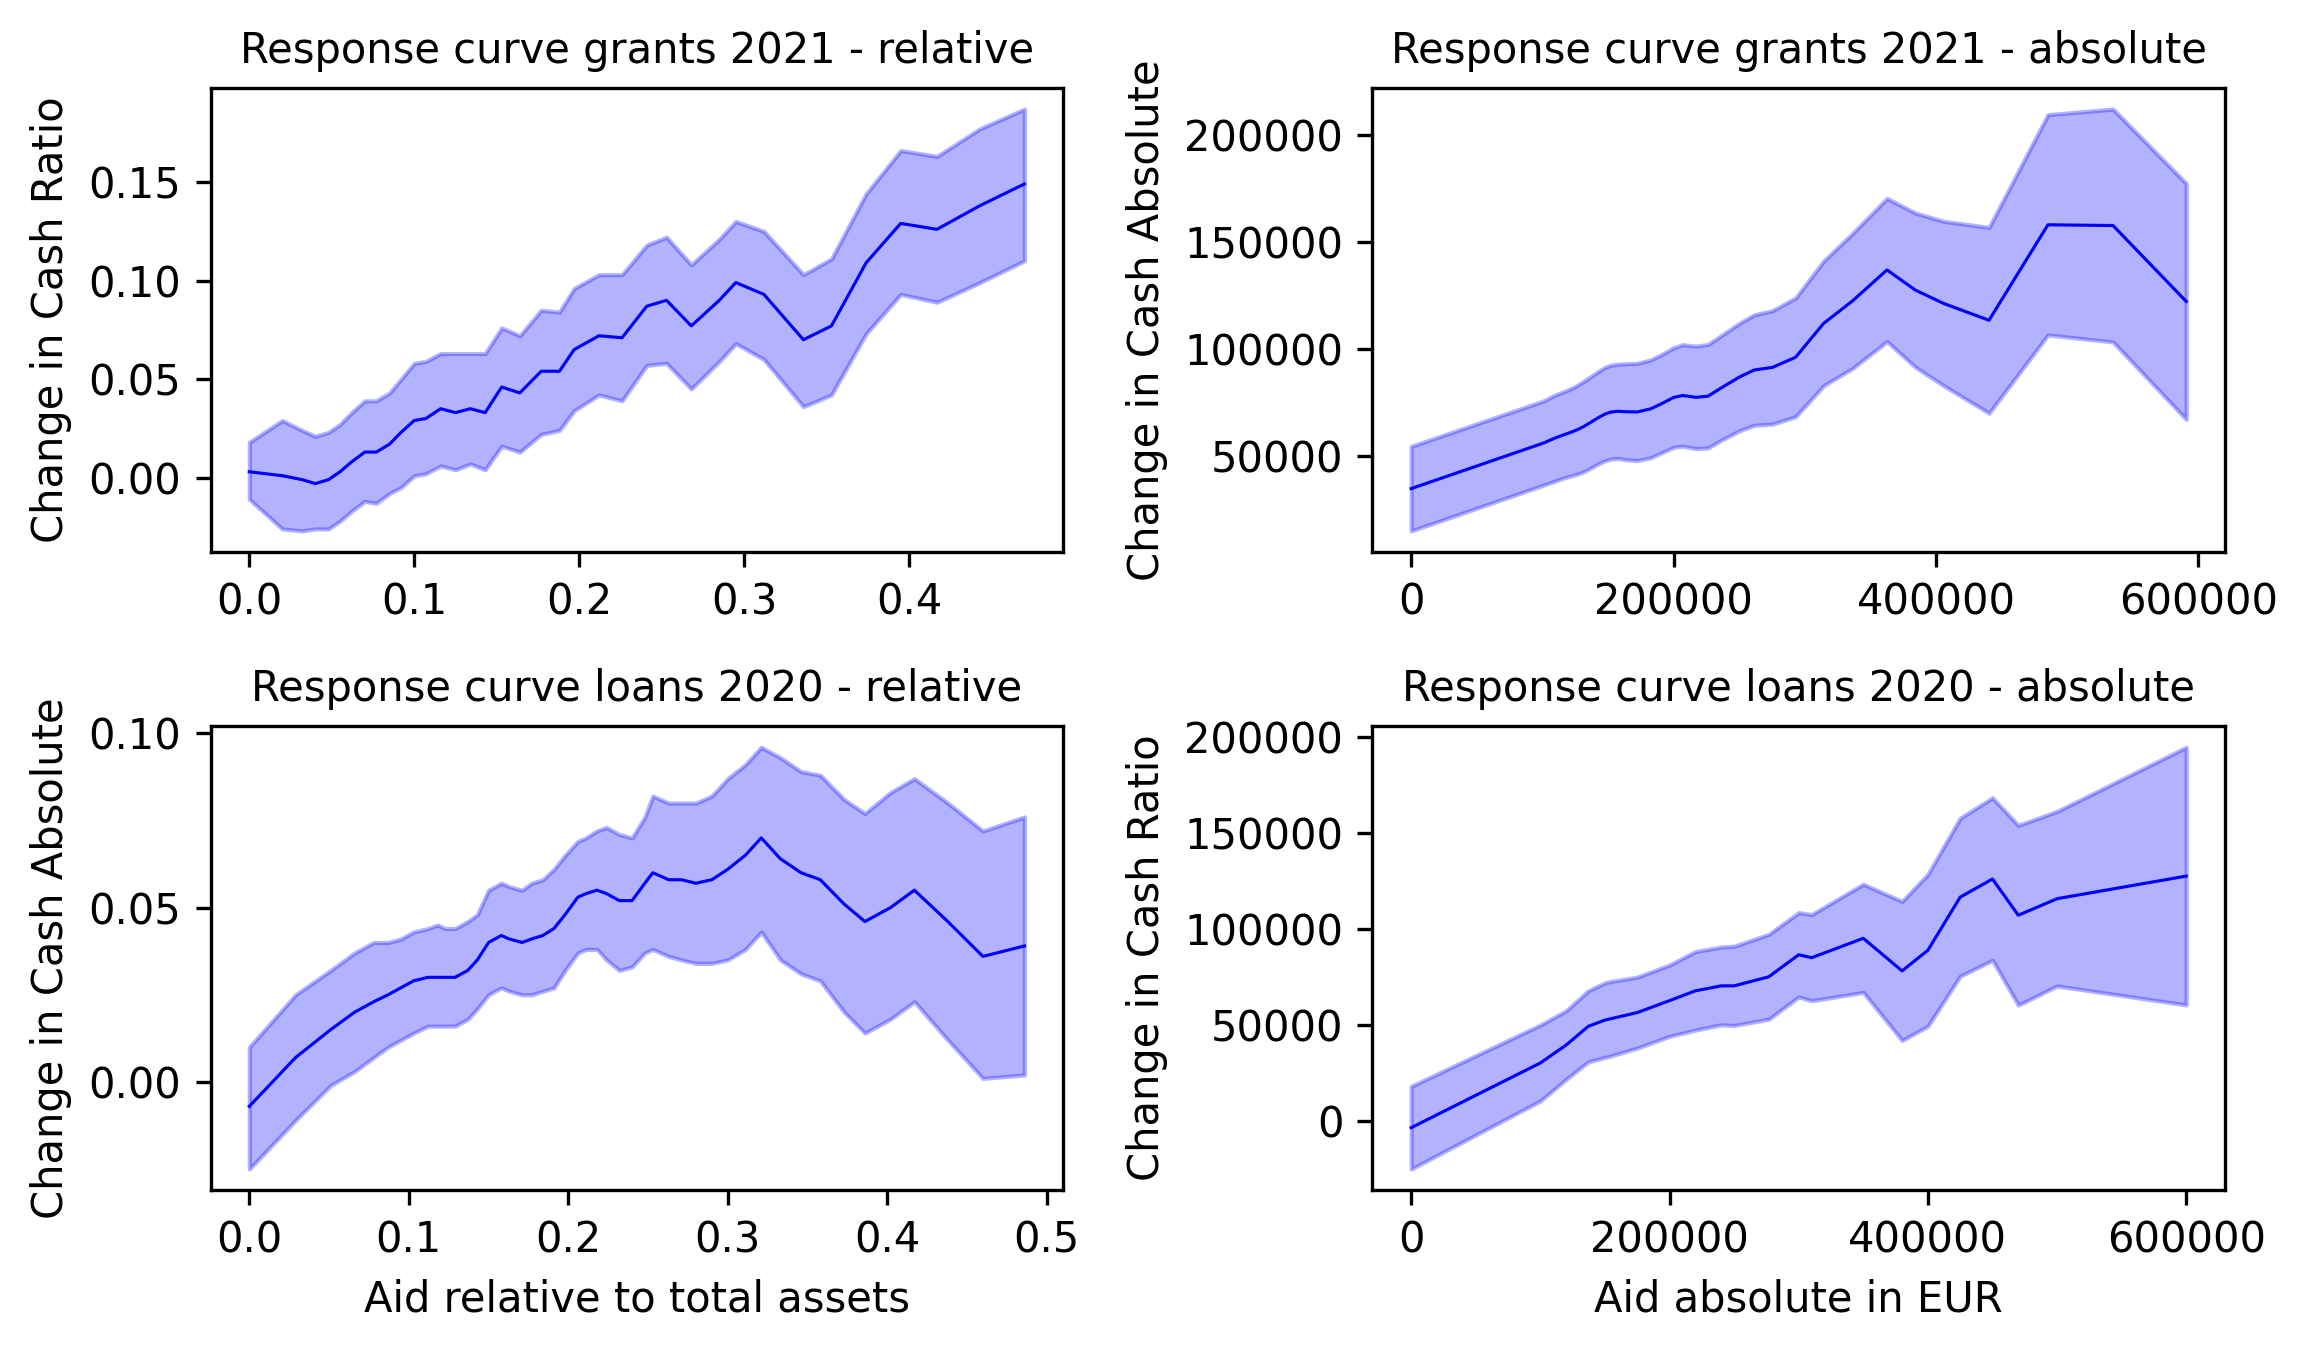
\includegraphics[width=1\columnwidth]{Figures/causal_curves1_raw.png}}
    
    \decoRule
    \caption[Response curves for grants and loans uncut]{Estimated Dose Response Functions, for liquidity (cash) from grants 2021 (top) and loans 2020 (bottom) in relative (left) and absolte (right) terms with 95\% Confidence Bands. For Binomial Distributed Data. The estimate of absolute variants used a lognormal GLM for the GPS estimation due to the different distribution of the variables.}
    \label{fig:Curve1raw}
\end{figure}


% 2
\section{Figure 5.4 with full Axis range}

\begin{figure}
    \centering
    \makebox[\textwidth][c]{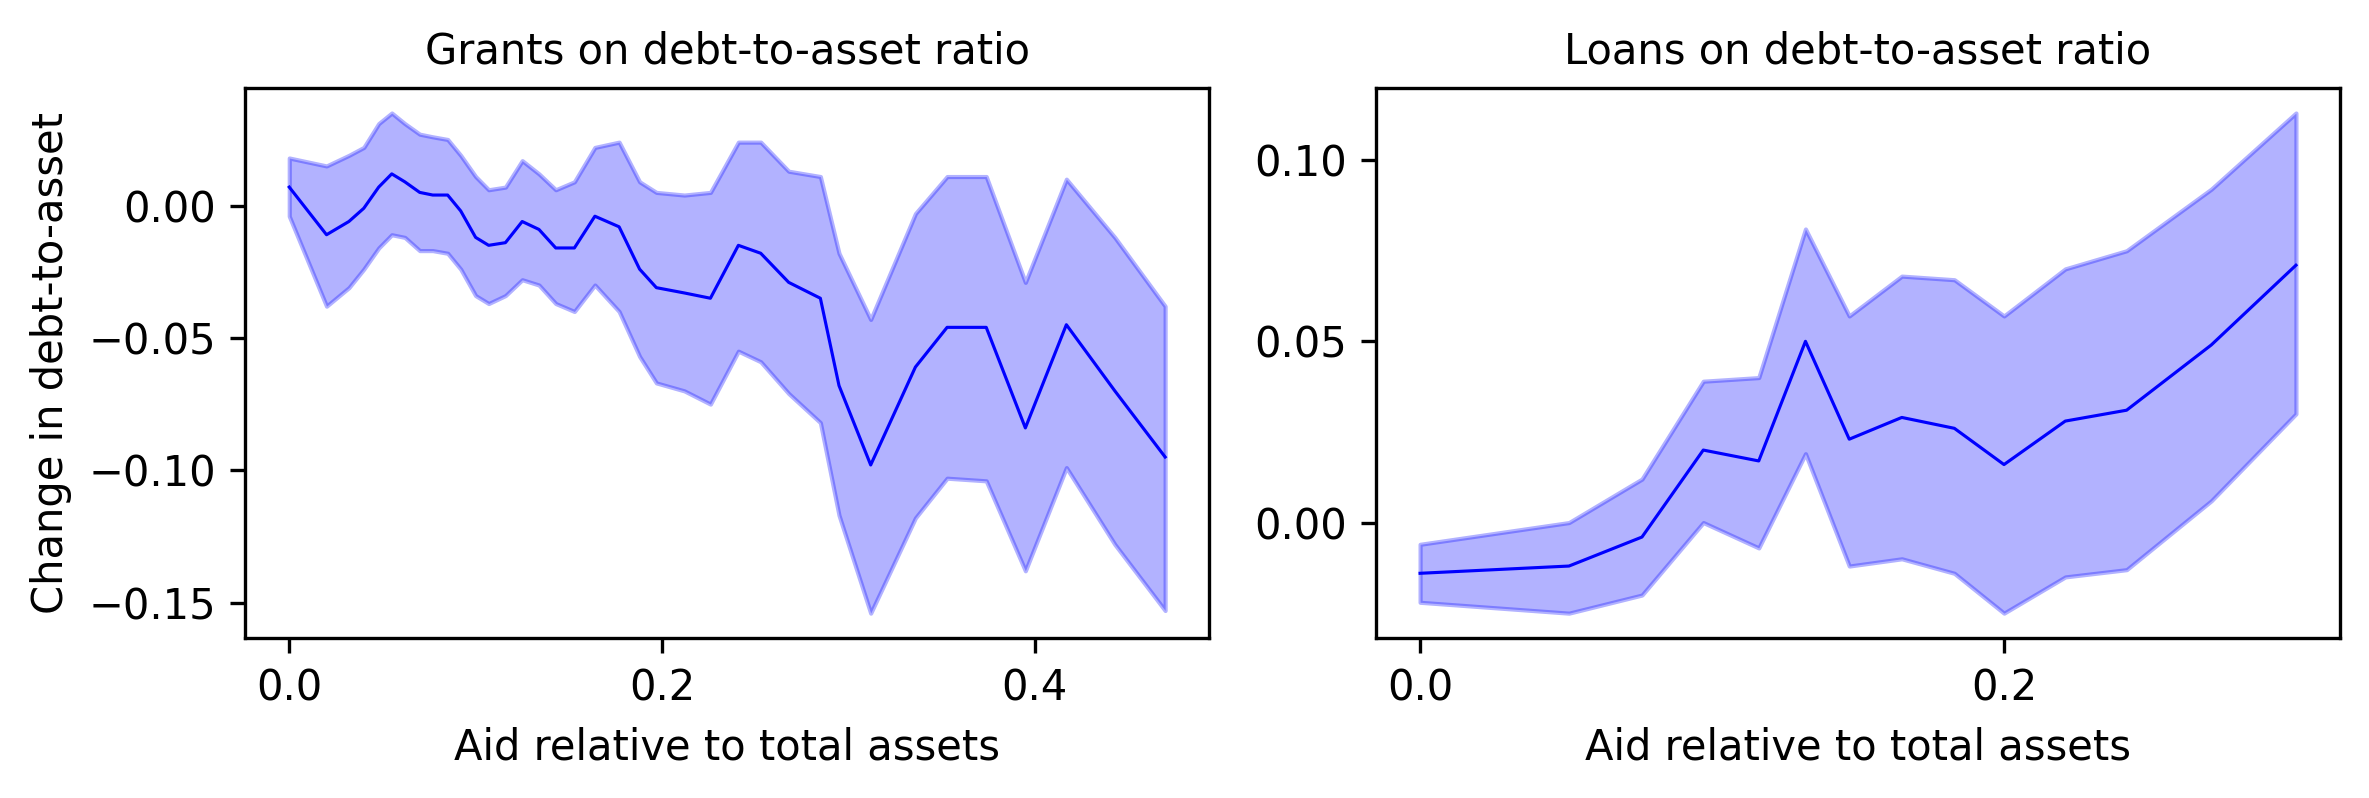
\includegraphics[width=1\columnwidth]{Figures/causal_curves2_raw.png}}
    
    \decoRule
    \caption[Response curves for indebtedness through aid uncut]{Estimated Dose Response Functions, for the debt-to-asset ratio from grants 2021 and loans 2021 in relative terms with 95\% Confidence Bands}
    \label{fig:Curve2raw}
\end{figure}



% 3
\section{Figure 5.5 with full Axis range}

\begin{figure}
    \centering
    \makebox[\textwidth][c]{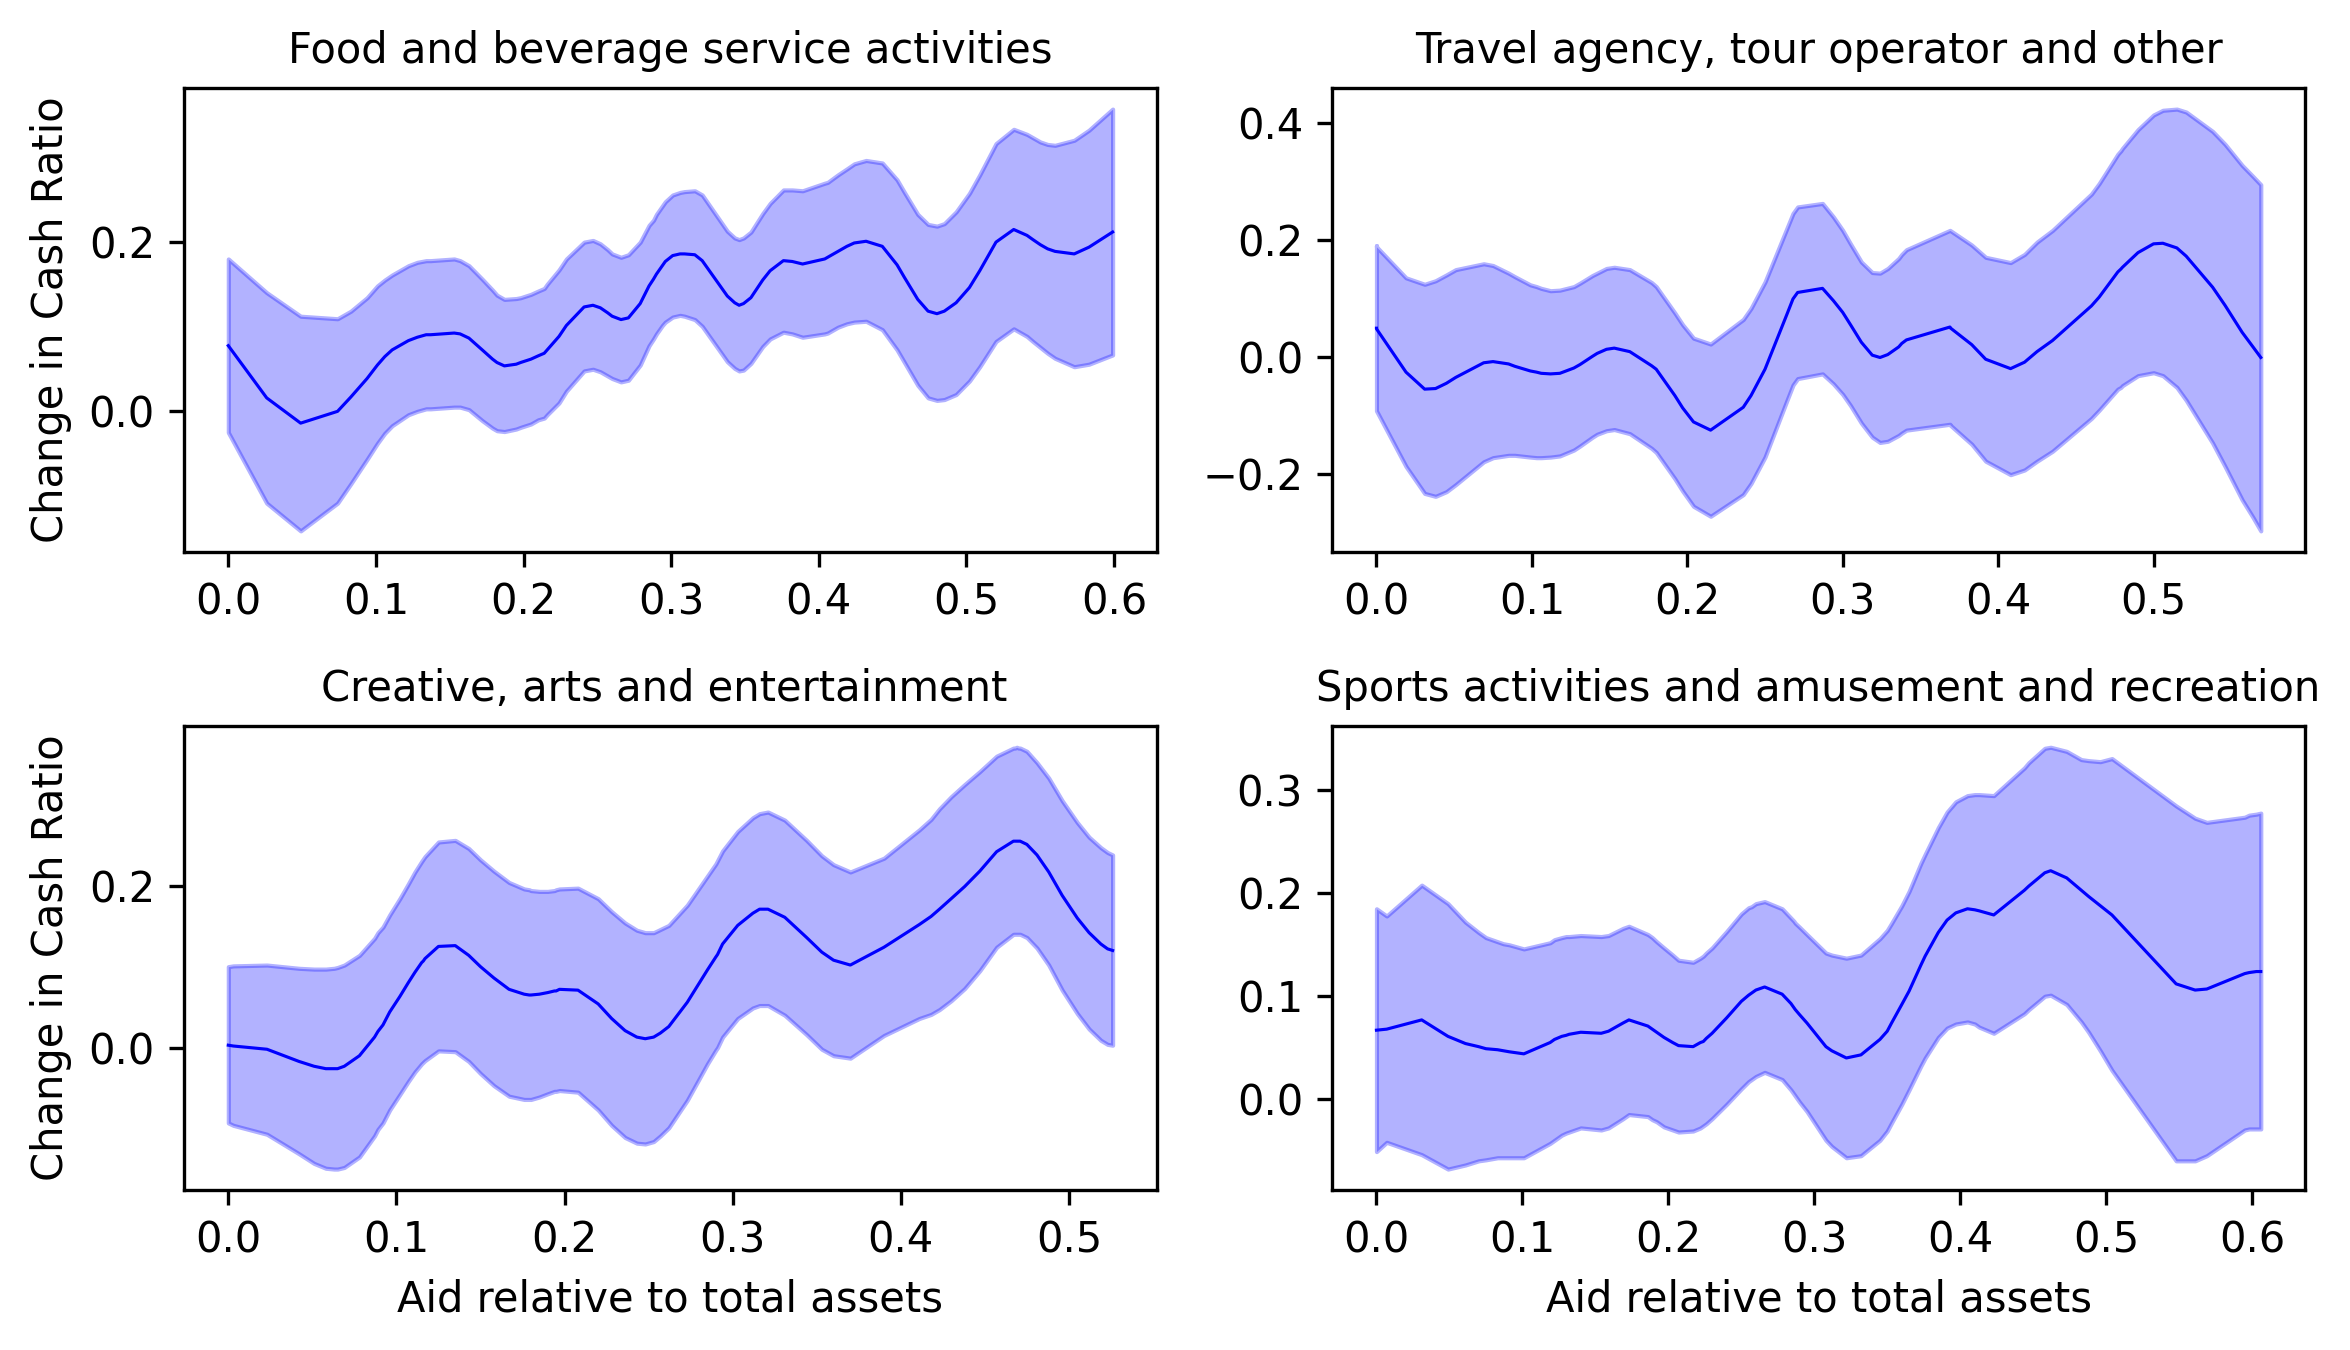
\includegraphics[width=1\columnwidth]{Figures/causal_curves_industries1_RAW.png}}
    
    \decoRule
    \caption[Response curves for liquidity through aid - by sectors 1 uncut]{Estimated Dose Response Functions, for the cash ratio from grants 2021 in selected industries in relative terms with 95\% Confidence Bands}
    \label{fig:Curve3raw}
\end{figure}



% 4
\section{Dose curves from addtional industries}

\begin{figure}
    \centering
    \makebox[\textwidth][c]{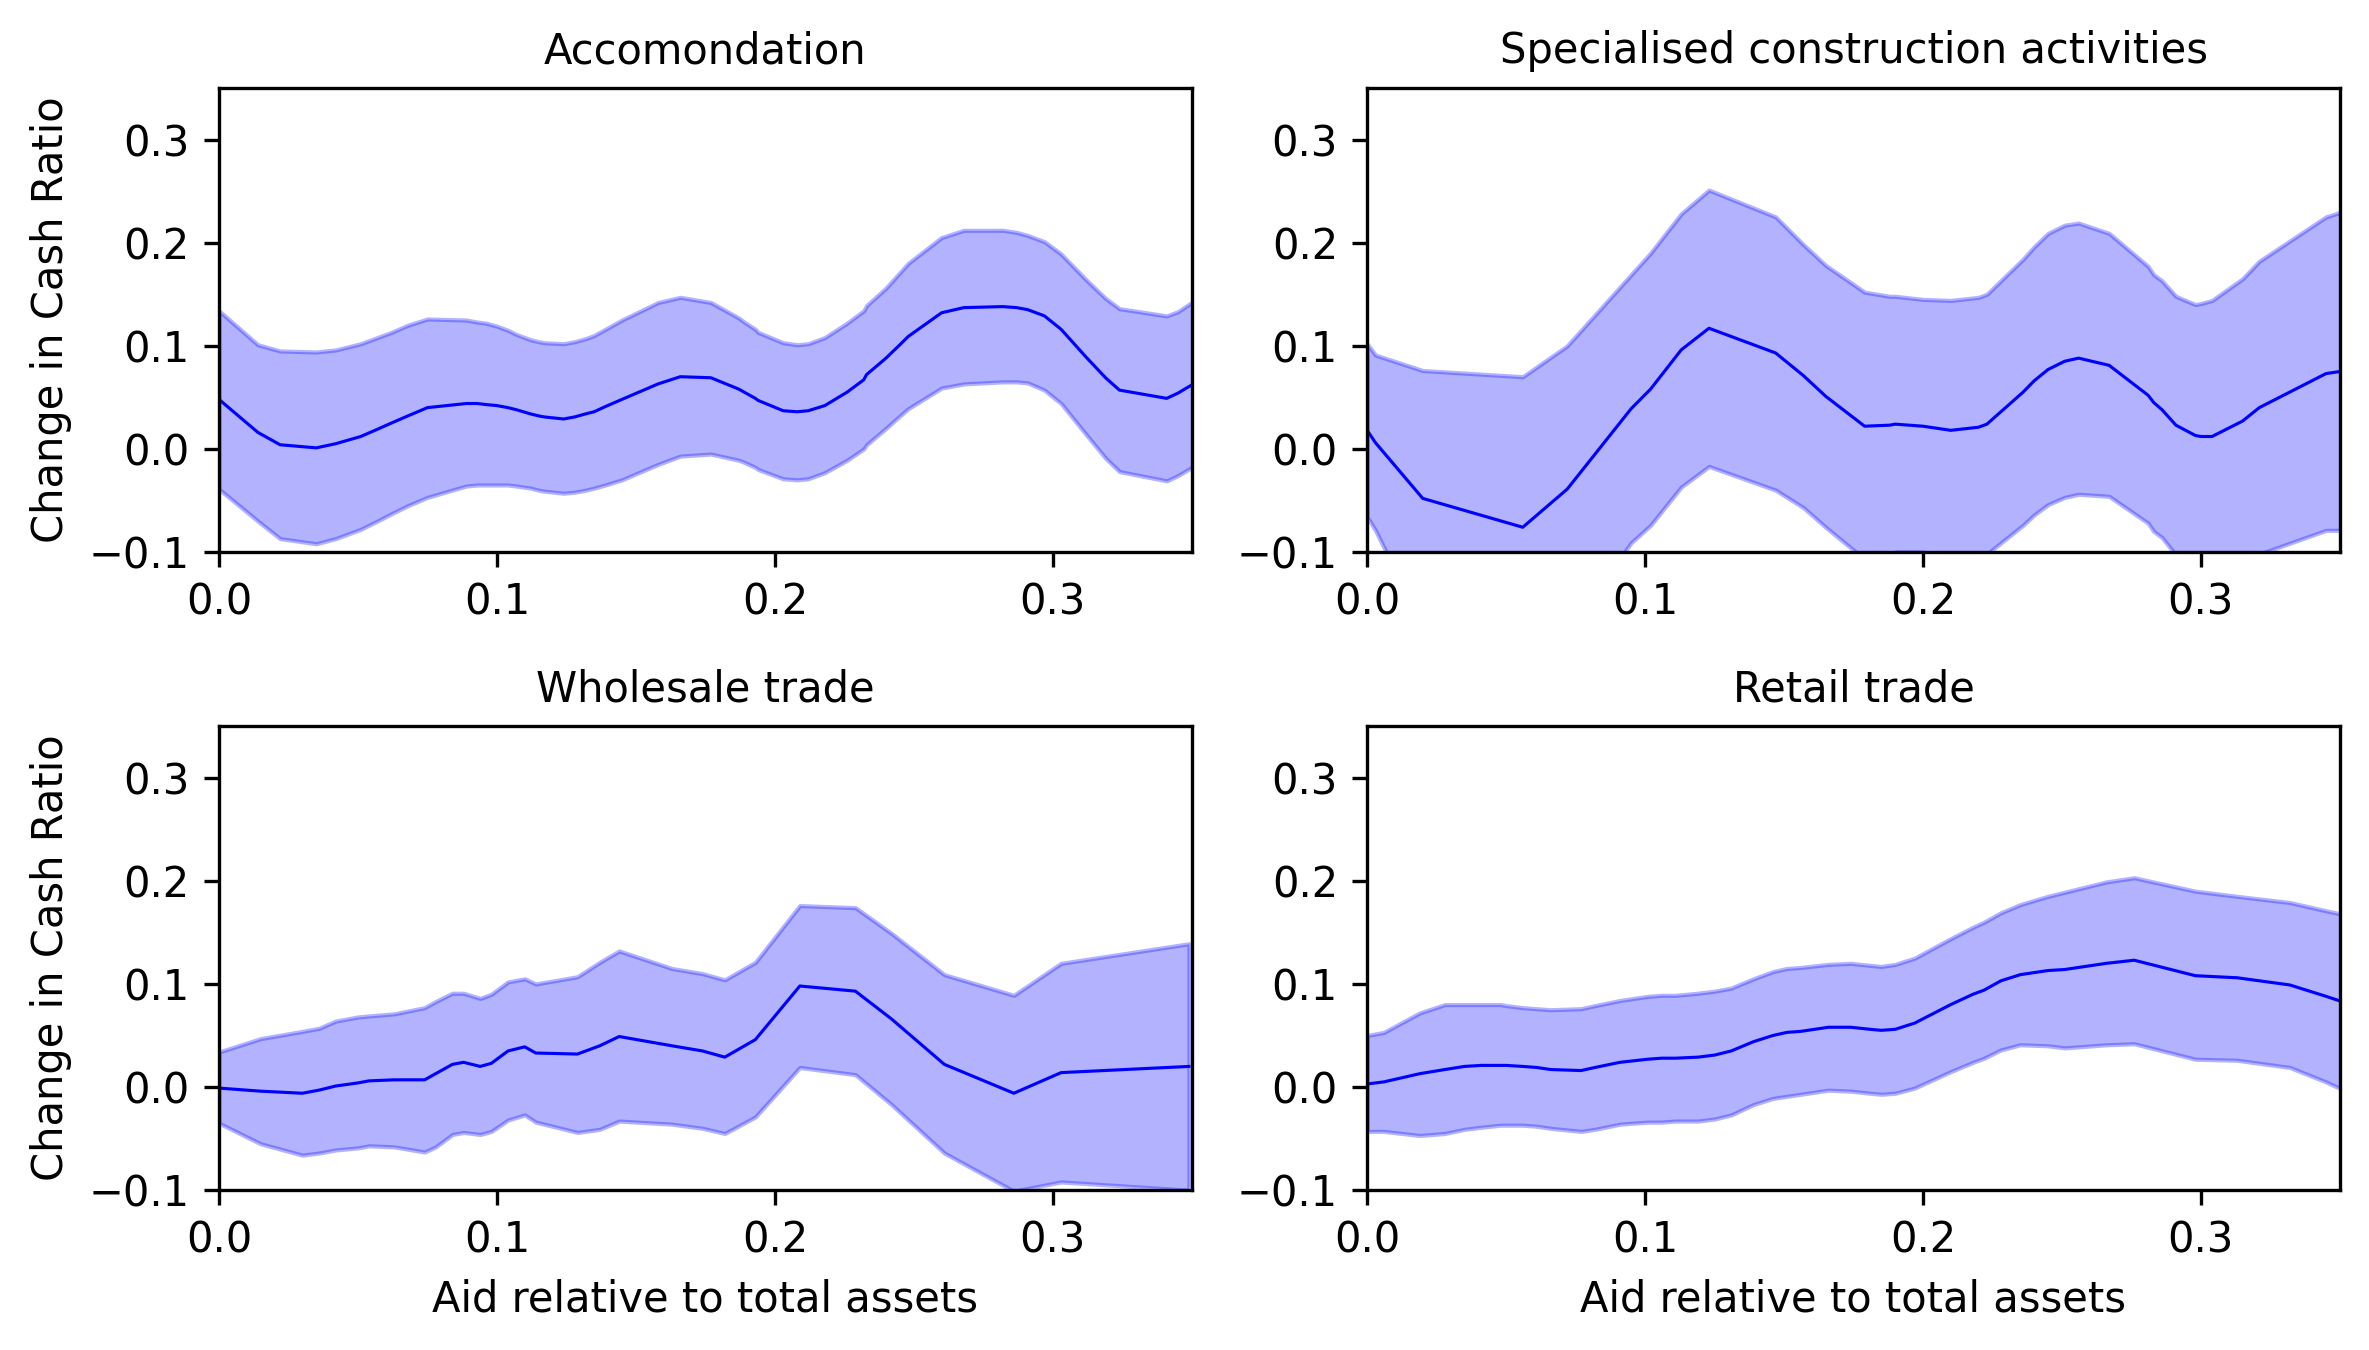
\includegraphics[width=1\columnwidth]{Figures/causal_curves_industries2.png}}
    
    \decoRule
    \caption[Response curves for liquidity through aid - by sectors 2]{Estimated Dose Response Functions, for the cash ratio from grants 2021 in selected industries in relative terms with 95\% Confidence Bands}
    \label{fig:Curve5}
\end{figure}

\begin{figure}
    \centering
    \makebox[\textwidth][c]{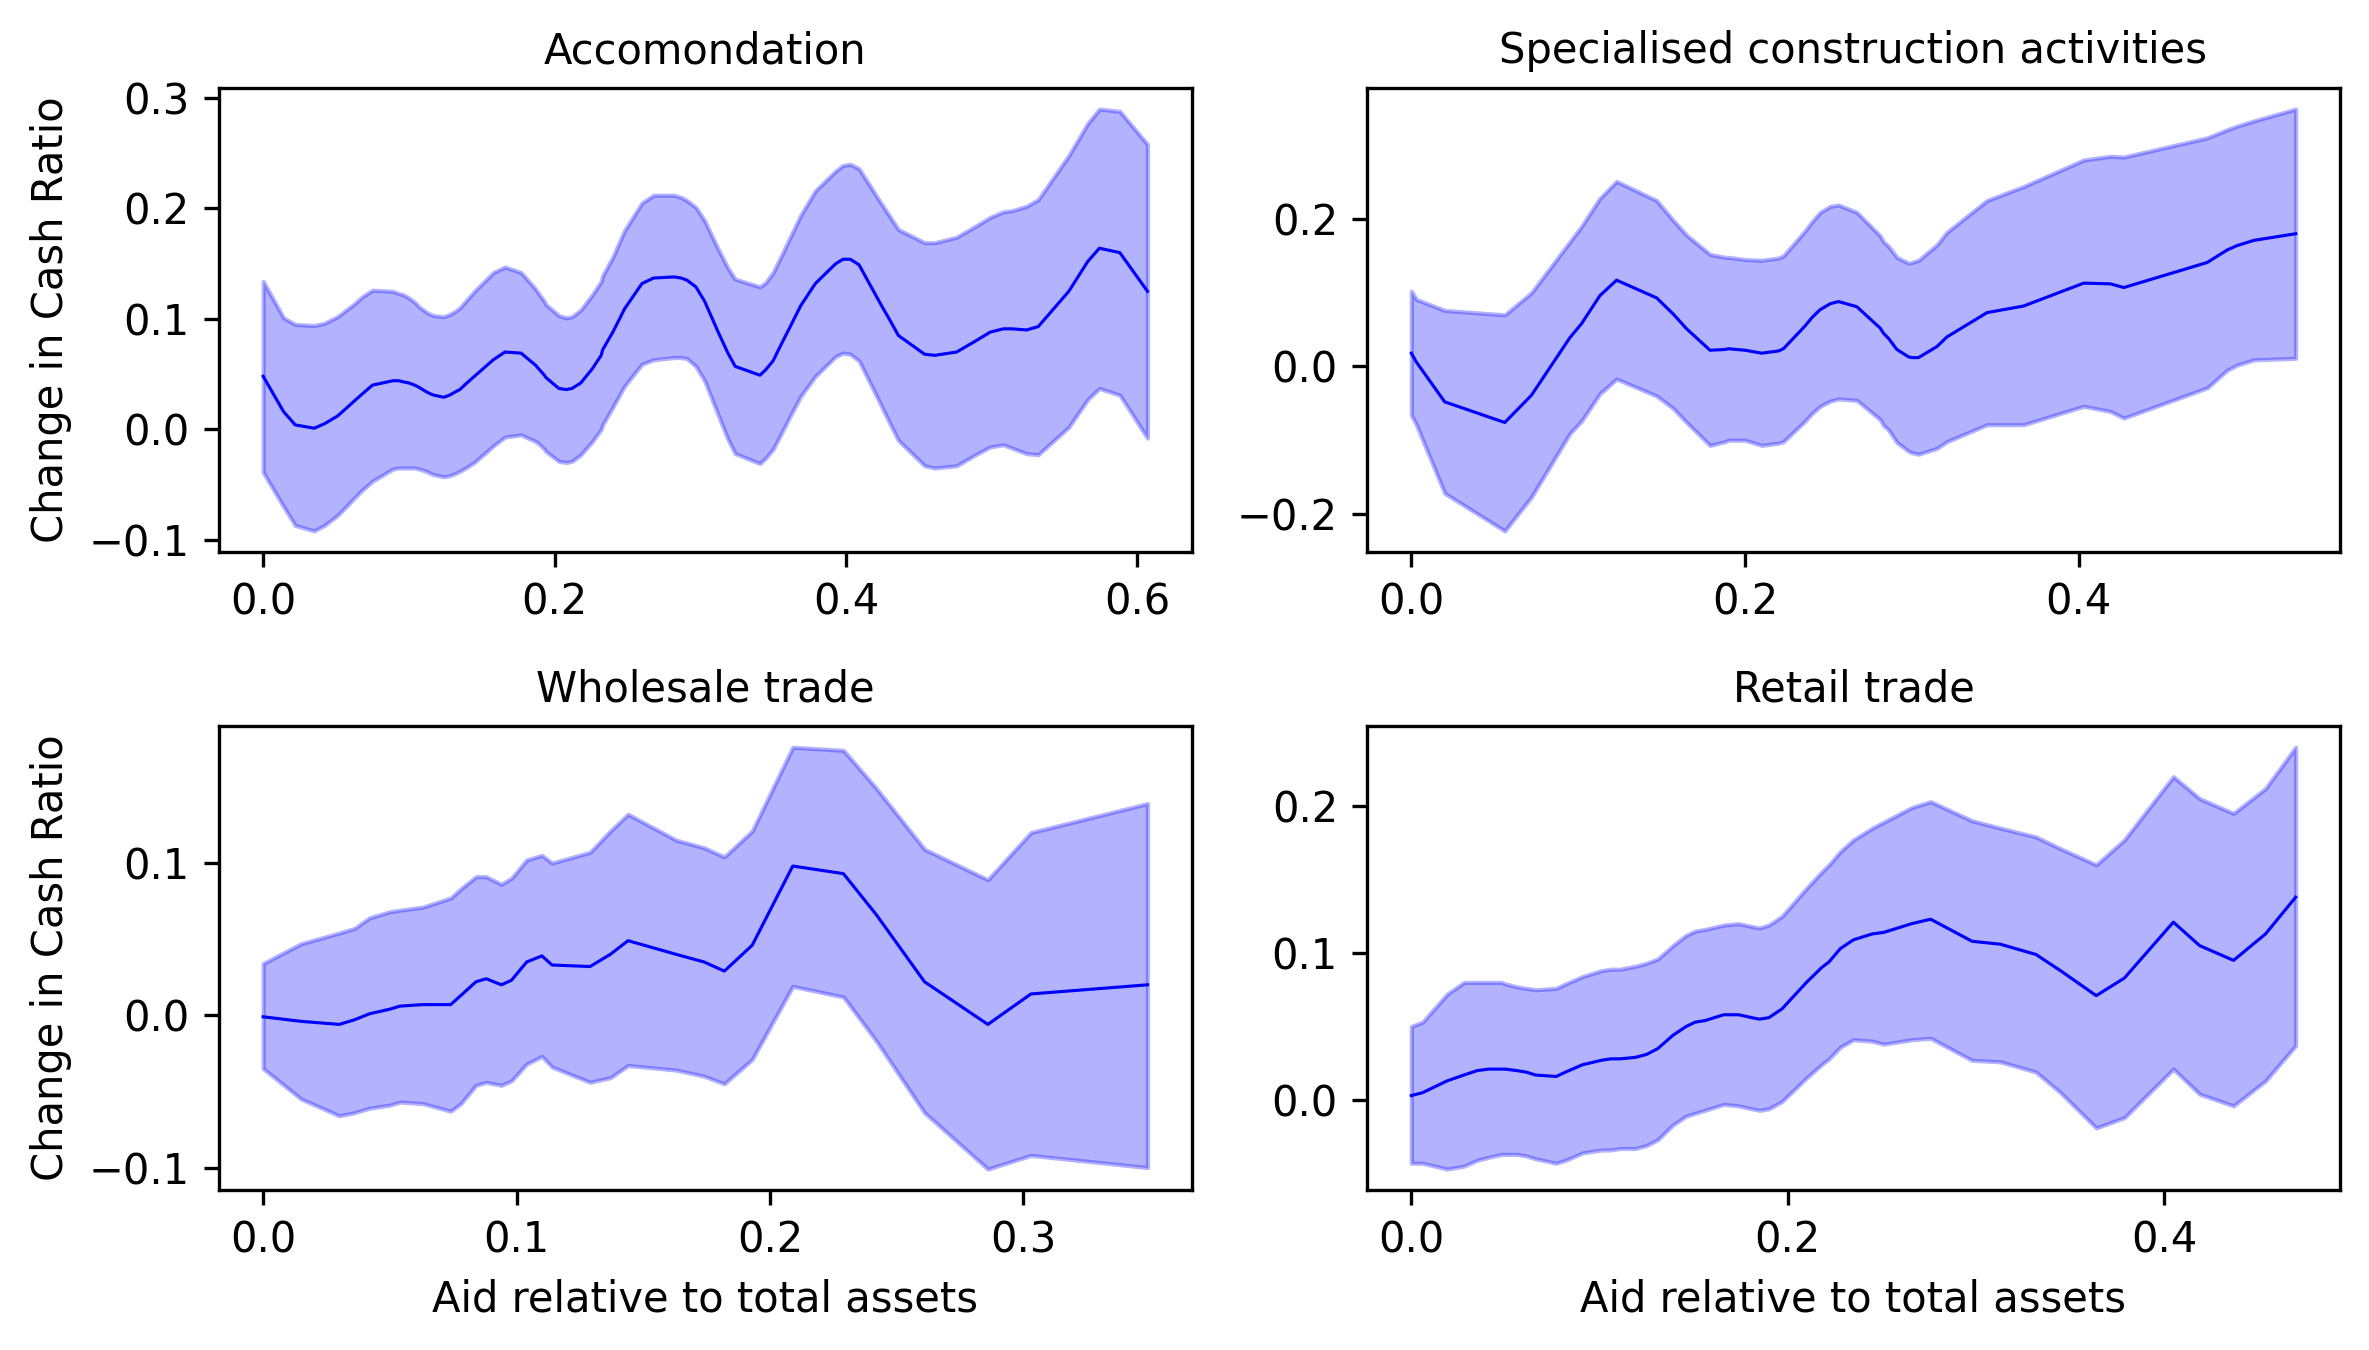
\includegraphics[width=1\columnwidth]{Figures/causal_curves_industries2_raw.png}}
    
    \decoRule
    \caption[Response curves for liquidity through aid - by sectors 2 uncut]{Estimated Dose Response Functions, for the cash ratio from grants 2021 in selected industries in relative terms with 95\% Confidence Bands}
    \label{fig:Curve5raw}
\end{figure}

%----------------------------------------------------------------------------------------
%	BIBLIOGRAPHY
%----------------------------------------------------------------------------------------

\printbibliography[heading=bibintoc]

%----------------------------------------------------------------------------------------
\def\authorshipname{Statement of Authorship}
\begin{declaration}
	\addchaptertocentry{\authorshipname} % Add the declaration to the table of contents
	\noindent I hereby confirm and certify that this master thesis is my own work. 
	All ideas and language of others are acknowledged in the text. 
	All references and verbatim extracts are properly quoted 
	and all other sources of information are specifically and clearly designated. 
	I confirm that the digital copy of the master thesis that 
	I submitted on 02.05.2023 is identical to the printed version 
	I submitted to the Examination Office on 03.05.2023.\\
	 
	\noindent DATE:\\
	%\rule[0.5em]{25em}{0.5pt} % This prints a line for the signature
	 
	\noindent NAME:\\
	%\rule[0.5em]{25em}{0.5pt} % This prints a line to write the date

	\noindent SIGNATURE:\\
	%\rule[0.5em]{25em}{0.5pt} % This prints a line to write the date
	\end{declaration}


\end{document}  
